\chapter{热类木星统计性质} \label{chapter:data_stat}

\section{系外行星统计列表}

在引言部分 \S \ref{sec: exopftheory},我们曾提到在如今已探测的系外行星中,有一群周期
小于十天却拥有大于土星质量的行星种群,被称为热类木星\footnote{若按照热类木星的定义,
其准确叫法应为近距离类木星,因为行星的有效温度不仅仅与主星的距离有关,而且还与主
星的有效温度有关。}。为了研究此类行星的统计性质,本文汇总了知名的四大系外行星数据
库网站 \url{http://exoplanets.eu/}、\url{http://exoplanets.org/}、\url{http://
exoplanetarchive.ipac.caltech.edu/} 和 \url{http://openexoplanetcatalogue.com/} ,并整理出
比较统一规范的系外行星列表\footnote{\url{https://github.com/EXONJU/ExoPlanetList}}。如
图 \ref{fig:hrplanet} 与 图 \ref{fig:exoskydist} 所示,在这行星数目为 3701 的样本中,共有 
375 颗系外热类木星系统(后文简称 HJs)。系外行星在南北天球分布并没有太多不均匀性
(除了巡天观测密集的几个区域以外),而 HJs 却在巨星分支中出现概率偏小(在 \S 
\ref{sec:hjofgiants} 中讨论),且大多数集中在类太阳恒星周围(下文介绍此为观测选择效
应)。本章节后续分析将统一建立在此 HJ 列表的范畴内讨论。

\begin{figure}
\centering
\includegraphics[width=1.0\textwidth]{figures/chapter4/fig2_HRplanet.pdf}
\caption{已确认系外行星的色指数与光度分布图,墨蓝色点为伊巴古星表临近太阳 150 pc 以内的恒星(图 \ref{fig:hrdiagram}),红五角星为太阳,绿色与黄色点如图 \ref{fig:exoskydist},被探测到的系外行星以及热木星明显集中在类太阳恒星附近,为观测选择效应。}
\label{fig:hrplanet}
\end{figure}


\begin{figure}
\centering
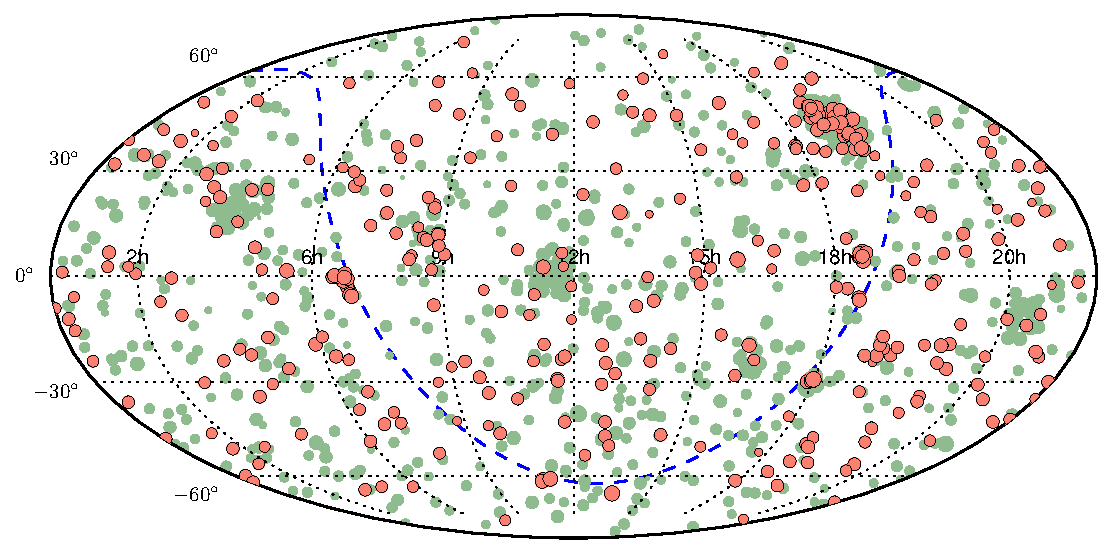
\includegraphics[width=1.0\textwidth]{figures/chapter4/fig1_exodistmollweide.pdf}
\caption{已被确认的系外行星在赤道坐标下的天球分布。图中蓝色虚线为银道面,可以看到巡天一般会远离银盘面(CoRoT 与 OGLE 除外)。绿色点为所有行星,黄色点则为热木星,点大小正比于 V 波段星等,从此图未见南北天的观测选择效应,$Kepler$ 视场(RA=19h 22m 40s,Dec=+44$^\circ$ 30' 00'' )为已确认系外行星最密集的区域之一。}
\label{fig:exoskydist}
\end{figure}


\section{HJs 出现概率}  \label{sec:hjoccurate}

按照已有的数据,现今探测到的 HJ 总数目约占已确认行星的 10\% 之多,这也是为什么
在图 \ref{fig:exomassper} 中,明显可以观察到一群质量在木星质量周期小于十天的行星
族。然而这与观测的选择效应密不可分。一个完备的统计必须建立在限定体积样本(
Volumn-limited sample)之上(文献 \citen{WinnFabrycky2015})。在一个限定体积的样
本中,热木星出现的概率并不高。Cumming 等人于 2008 年对 RV 巡天中的 600 颗 FKGM 
恒星监测了 8 年后的结果显示\cite{Cumming2008},对于 $M_\tif{p} > 100 \tif{M}_\oplus,\, 
P<5.5$ years 的行星的出现概率可用如下公式描述:

\begin{equation} \label{eq:pltoccurate}
\frac{\tif{d} N}{\tif{d}\ln M_\tif{p} \tif{d}\ln P} \propto  M_\tif{p}^\alpha P^\beta \ \, ,
\end{equation} %myequation{行星出现数目的概率分布}
其中指数 $\alpha = -0.31 \pm 0.20 $,$\beta = 0.26 \pm 0.10$。结合其他种类的巡天项目,
对应的 HJs 的出现概率大致为 0.5 \% 到1.5 \% 之间不等\cite{Howard2012,Marcy2005,
Mayor2011,Wright2012}。此概率的不同和恒星的星族选择密切相关\cite{Wright2012},比如
恒星的金属丰度和类木星出现的概率有明显的正相关性\cite{Gonzalez1997,Santos2001,
Santos2004,Fischer2005,Udry2007,Sozzetti2009,Sousa2011},这也恰好佐证了 \S 
\ref{sec:clspftheory} 中描述的气巨星重元素核吸积模型。


\section{HJs 形成} \label{sec:hjform}


在传统的核吸积模型中\cite{IdaLin2004b},气巨星往往需要在距离主星几个天文单位的地方
才能有足够多的原材料(绝大部分由冰组成)供固态核形成。然而在观测中,HJs 的统计
分布于 3 天附近存在峰值(见图 \ref{fig:hjperecc})。因此需要解释 HJ 的形成,大致上有
两大种方法:在传统的行星形成基础上引入木星的轨道迁移(\textit{orbital migration})或
直接于当地形成(\textit{in situ. formation})。关于热木星的本地形成请参见文献 
\citen{Batygin2016},本文分析的主要讨论对象为前者。

\begin{figure}[t]
\centering
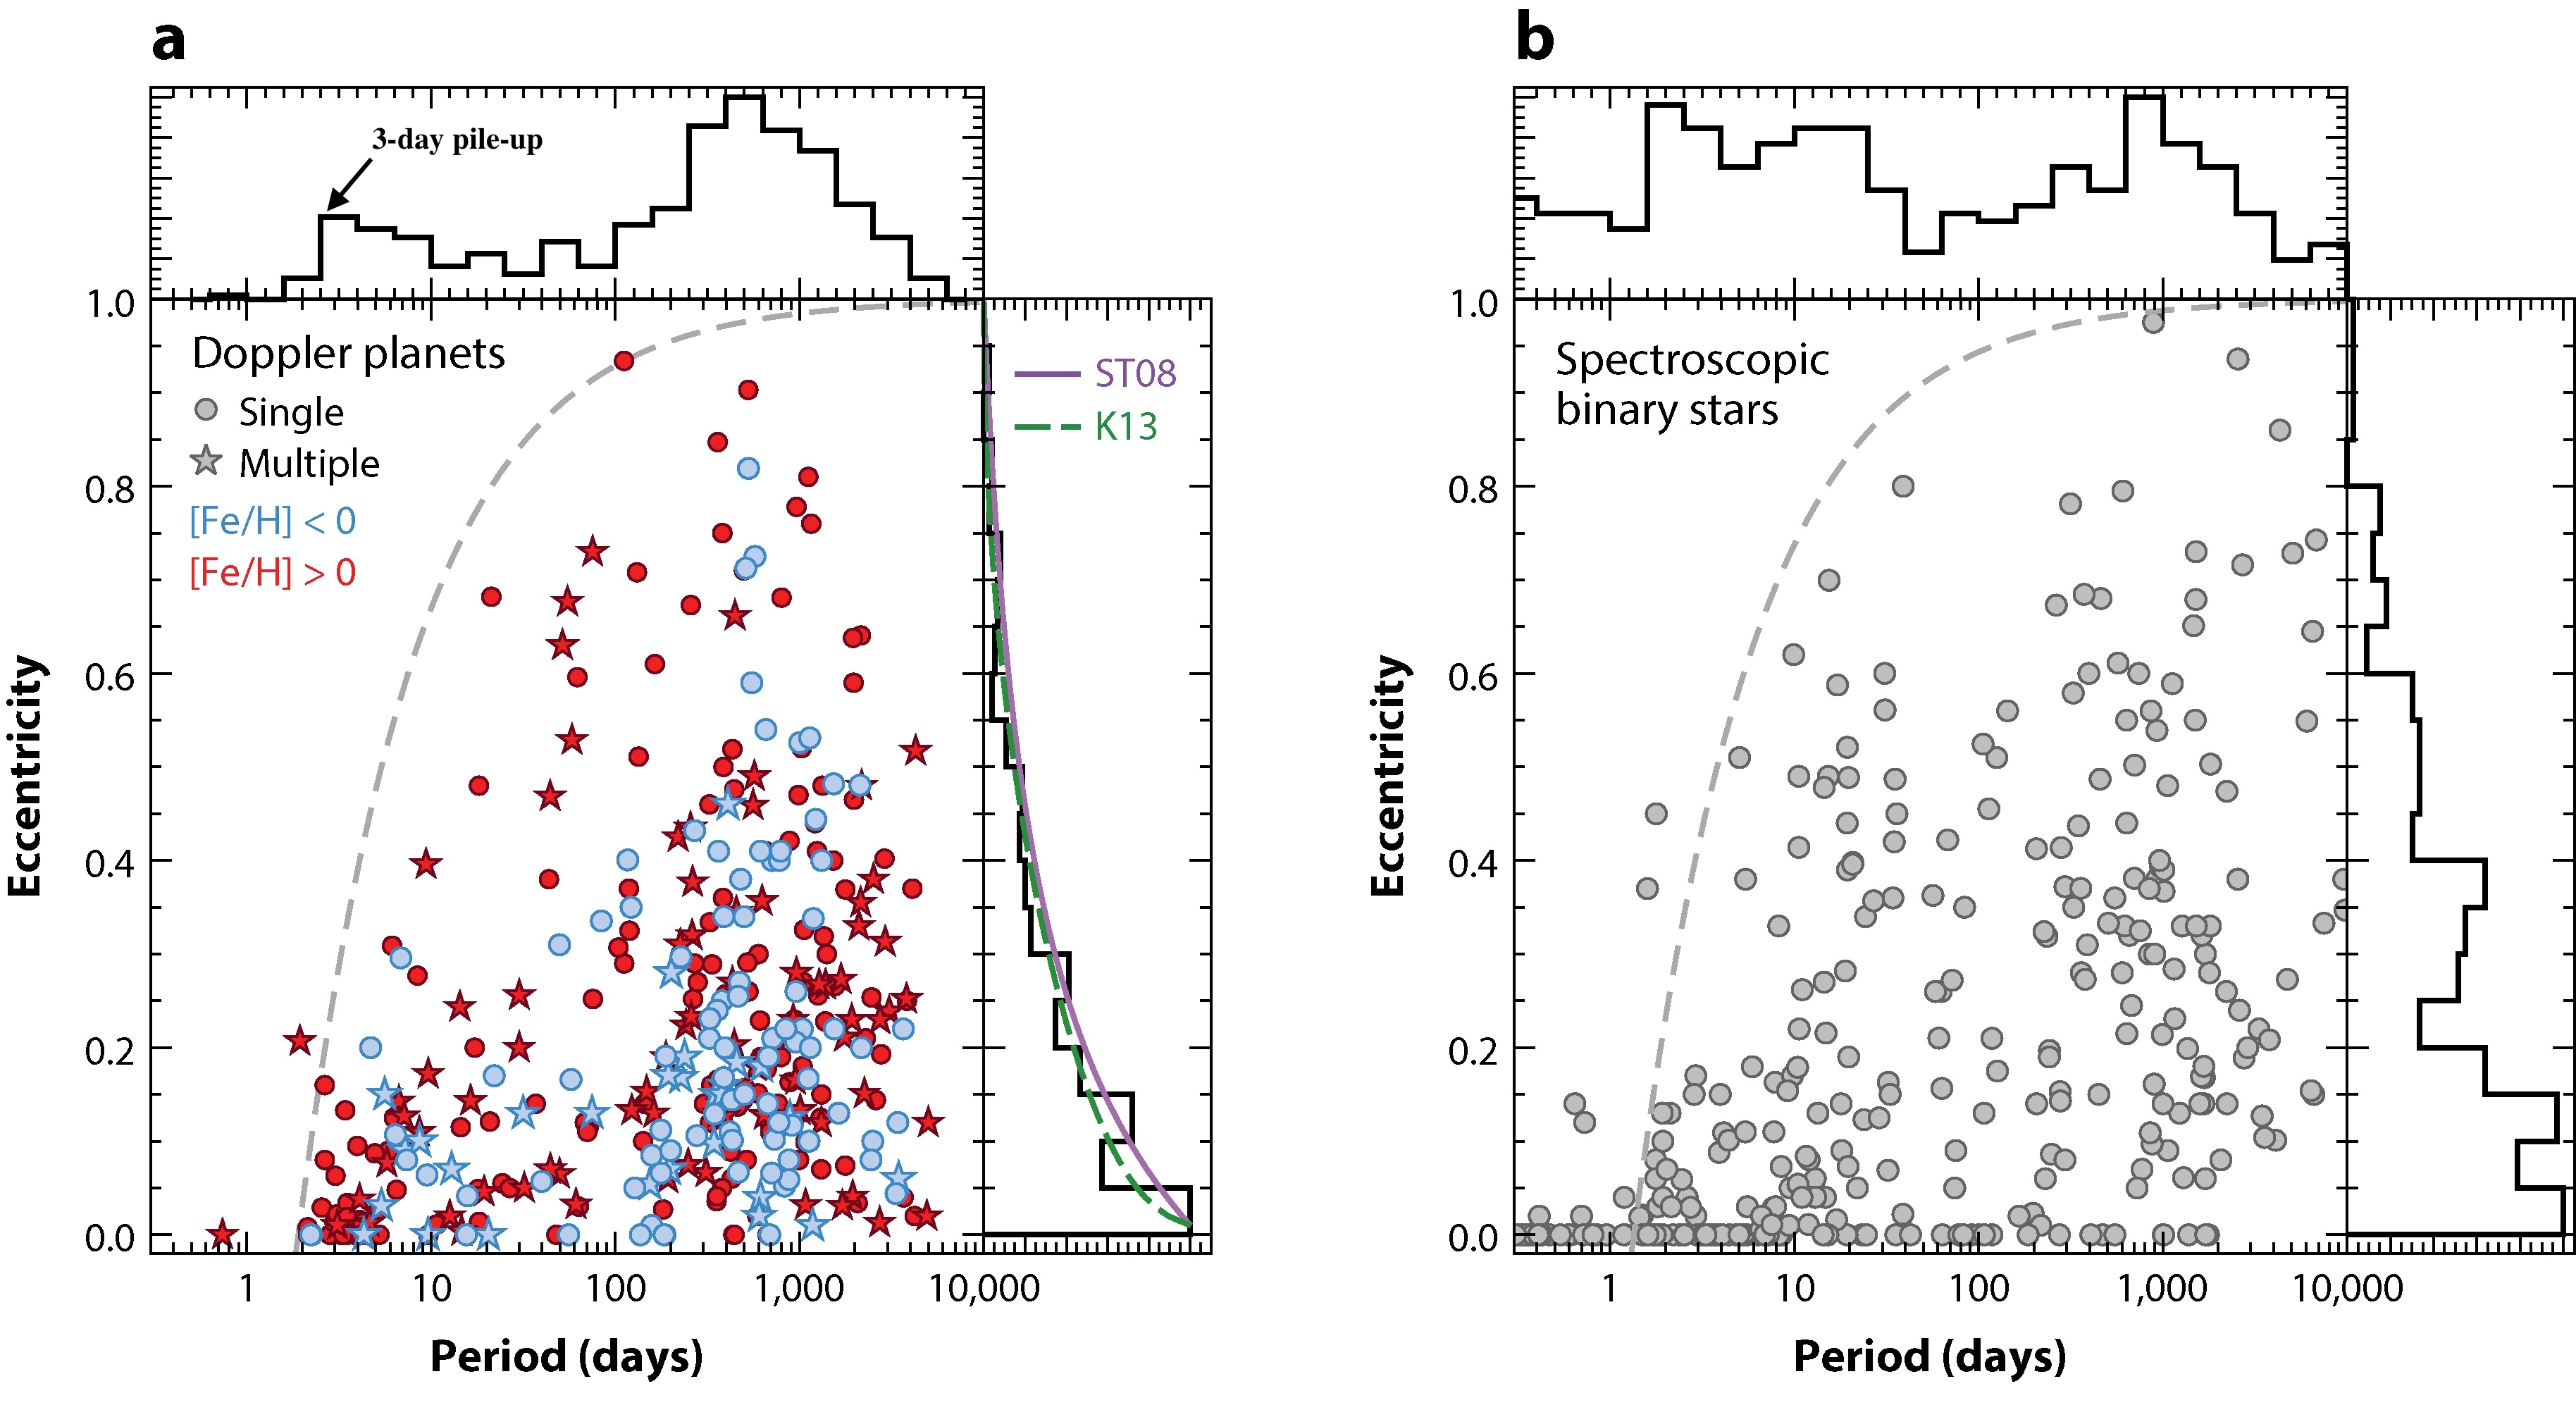
\includegraphics[width=1.0\textwidth]{figures/chapter4/fig3_peccdist.jpeg}
\caption[热类木星系统的周期与轨道偏心率分布图。可以看到系外行星样本(未经过选择效应修正)在三天周期分布达到热类木星的峰值,虚线为类太阳恒星周围行星拥有近心点距离 $a(1-e) = 0.03$ AU 的轨道。右侧图为 SB9 光谱双星星表的类似分布图,图片取自 Winn 和 Fabrycky。]{热类木星系统的周期与轨道偏心率分布图。图片取自文献 \citen{WinnFabrycky2015},可以看到系外行星样本(未经过选择效应修正)在三天周期分布达到热类木星的峰值,虚线为类太阳恒星周围行星拥有近心点距离 $a(1-e) = 0.03$ AU 的轨道。右侧图为 SB9 光谱双星星表的类似分布图。}
\label{fig:hjperecc}
\end{figure}


\subsection{轨道迁移} \label{sec:migration}

在传统的行星形成的基础上,行星的轨道迁移并不需要引入额外的行星核心生长以及气体
吸积机制。轨道迁移代表着轨道半长径 $a$ 发生了变化,在椭圆二体运动中行星的角动
量与能量拥有如下表达式(本文内均假设 $M_\tif{p} \ll M_\tif{s}$):

\begin{eqnarray}
E = - M_\tif{p} \, \frac{\mu}{2a} \\ \label{eq:2be}
J = M_\tif{p} n a^2 \label{eq:2bam}
\end{eqnarray} %\myequation{二体运动中的能量与角动量}
其中 $n$ 为平均轨道角速度,满足开普勒第三定律 $n^2a^3=\mu$,其中$\mu = G M_\tif{s}$
如此轨道迁移势必意味着角动量(Angular Momentum,简称 AM)与能量的交换,因此必须
有其它物体与行星之间发生 AM 与能量传递。这样一来,我们又可将轨道迁移大致分为两
种情况:气体盘迁移(\textit{disk migration})和高偏心率迁移(\textit{high-e migration})。

\subsubsection{气体盘迁移} \label{sec:diskmig}

由于木星质量的行星核心形成后会依然嵌套在恒星周围的气体盘内,因而由于盘的气体和之
间会存在 AM 交换。这样的的 AM 交换通常是通过处于 Lindblad 共振的气体的 co-rotational 
力矩来实现\cite{Binney1987,GoldreichTremaine1979},比如土星环的结构
\cite{GoldreichTremaine1980}。简单来说第 $m$ 阶共振距离主星半径与行星轨道之间的关系
为 $r_\tif{L} = (1\pm 1/m)^{2/3} a_\tif{p}$。在二体问题中希尔半径(或洛希半径)可描述为:

\begin{equation} \label{eq:hillradius}
r_H = \big( \frac{M_\tif{p}}{3M_\tif{s}} \big) ^{1/3}
\end{equation} %myequation{希尔半径(或洛希半径)表达式}

如果行星的质量足够大,使得希尔半径大于盘的标高($r_H > h$),那么盘可能被被打开缺
口。与此同时,由于气体盘的粘性,此缺口也可能被气体重新填上。1986 年,Lin 等人通过
比较盘缺口由于粘性重新被填补上以及由于 Lindblad 共振又再被打开的时标,得出在经典的
原行星盘参数下,木星质量的行星足以打开空缺,而土星的质量则约为打开空缺的临界值
\cite{Lin1986,Ward1997}。后来该理论被成功地在人类发现的第一颗类太阳系外 HJ --- 51 Peg
 b 上\cite{Lin1996},比如在 5 AU 附近的木星,在标准的行星盘打开缺口后,将在时标为 0.5 
 Myr 左右迁移至原行星盘的内边界。这样的气体盘迁移又被称作第二型(Type II)轨道迁移
 (见图 \ref{fig:diskmig})。

\begin{figure}[t]
\centering
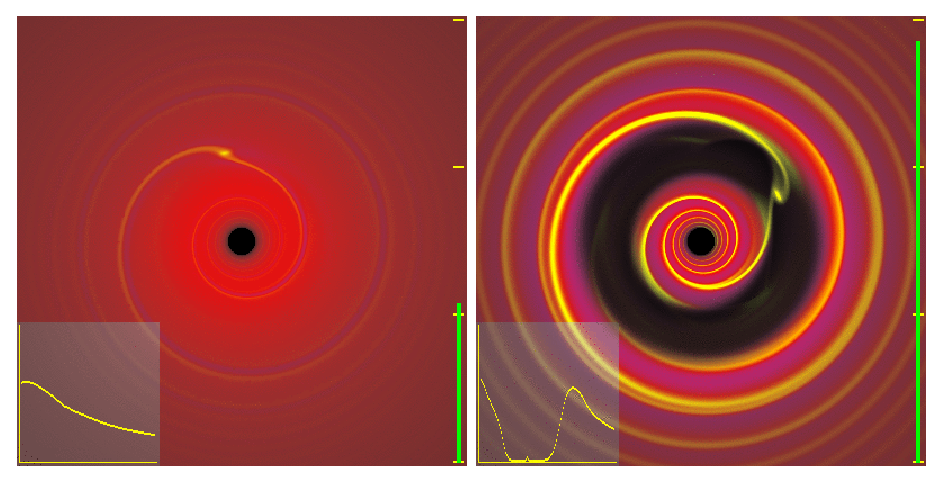
\includegraphics[width=1.0\textwidth]{figures/chapter4/fig3_diskmig.eps}
\caption[典型的第二型轨道迁移数值模拟,大质量行星可以在盘内打开空缺,并且往靠近恒星的盘内侧迁移。图片版权 Armitage\/Rice。]{典型的第二型轨道迁移数值模拟,大质量行星可以在盘内打开空缺,并且往靠近恒星的盘内侧迁移。图片取自文献 \citen{Armitage2005}。}
\label{fig:diskmig}
\end{figure}


\subsubsection{高偏心率迁移} \label{sec:highemig}

行星在气体盘中的迁移往往会受气体的阻尼作用而不那么剧烈(保持小偏心率轨道来交换
AM)。相比之下,其它天体造成的引力扰动则会显得更为直接,之所以称此类作用为
高偏心率迁移也正是如此得名。一旦类木星的偏心率达到能使得其轨道近心点距离达到当
前观测 HJs 几天轨道周期的位置,那么潮汐演化便可将其作用成热木星(\S \ref{sec:tidal})。
高偏心率作用的天体可以是一群小天体(单个小质量的天体几乎不能改变木星),如散射
星子盘导致的行星迁移\cite{Malhotra1993,Murray1998,Morbidelli2007,Thommes2008},
或者更多的则是质量相当或更大天体的强引力扰动(如木星与土星的长期摄动
\cite{MurrayDermott1999ssd})。目前此类别下主流的解释因素包括以下几种:

\textbf{伴星级扰动}。早在 1962 年,木星的存在对高轨道倾角太阳系小天体的轨道影响就
已被提出\cite{Lidov1962,Kozai1962}。而后 Wu 和 Murray 于 2003 年将此 Lidov-Kozai 
效应效应引入解释系外热木星\cite{WuMurray2003},即当引入一颗行星系统外具有较大
轨道倾角的伴星时,行星的轨道偏心率(以及轨道倾角)会发生周期性的 Kozai 共振
\cite{Innanen1997}。然而观测中伴星存在的概率是否能解释所有的 HJ 系统\cite{Wu2007,
Fabrycky2007},共振的最高偏心对伴星的质量和轨道要求也值得进一步讨论\cite{
Naoz2011,Nagasawa2011}。甚至在恒星形成的星团环境中,其它天体的飞掠(flyby)也
可能会对行星系统造成一定的影响\cite{Spurzem2009}。

\textbf{行星级扰动}。多行星系统内行星之间无处不存在着扰动,如果行星之间动力学足够
不稳定,那么可能发生行星---行星散射(planet-planet scattering 简称 PPS,参见文献
\citen{Rasio1996a})。对于一般有规律并排(orderly spaced)的行星系统,动力学作用
会产生中等偏心率的行星\cite{Zhou2007,IdaLin2013,Lin1997,Juric2008,Chatterjee2008},
而若要产生能够形成 HJs 的大偏心率,则需要长期作用下的混动效应\cite{Wu2011}。

另外,形成热木星高偏心率还有一些混合以上盘迁移以及高偏心率迁移的其他理论,详见
文献\citen{Weidenschilling1996,Nagasawa2008,Chen2013}。理论虽多,但迁移的总体思
路实则不变: 拥有能够与 HJ 交换 AM 的另外一颗天体以及整个系统初始的角动量亏损
(Angular Momentum Deficit,AMD)。正是如此才需要观测和统计去区分不同的物理作
用过程并且打破观测中不同理论的简并度(图 \ref{fig:pfenv})。


\section{引力潮汐作用} \label{sec:tidal}

前文提到在高偏心率迁移的框架下,需要额外引入潮汐过程才能解释如今观测到 HJs
几乎全体近圆的轨道统计分布(见图 \ref{fig:hjperecc})。在 51 Peg b 发现的第二年,
Rasio与 Ford 就意识到潮汐因素在 HJs 的形成演化中起了非常重要的作用\cite{Rasio1996b}。
而事实上,在近距离的二题问题中(轨道周期在几天附近),由于天体并非质点,因而
引力潮汐导致的形变效应的确是一项不可忽略的非开普勒(non-keplerian)作用项。潮
汐现象在我们太阳系甚至地月系统都很常见,月球的公转自转潮汐锁定,以及地球上海洋
的涨潮落潮,也都是潮汐的体现。现代的潮汐理论主要基于 Darwin 在 1880 年基于球谐函
数下对天体非开普勒引力势展开\cite{Darwin1880}:

\begin{equation} \label{gravipotential}
U(r) = \sum\limits_{l=2}^\infty \sum\limits_{p=0}^l\sum\limits_{q=-\infty}^\infty \frac{Gm}{a} A_{l,p,q}(e,\,\Psi)\big(\frac{r}{a}\big)^l Y_l^p(\theta,\,\phi) \tif{e}^{-\tif{i}q n t} \ .
\end{equation} %\myequation{非球形引力势展开}
各物理量的定义如图 \ref{fig:tideillu} 所示,$n$ 为平均轨道角速度,$a,e$ 为轨道根数
(有时也会用二体之间的距离 $d$ 来作为展开基数),$\Psi$ 为 $m$ 体轨道法向 $L$ 
与 $M$ 体自转法向的夹角( 又称 obliquity),$A_{l,p,q}$ 系数则依赖于天体 $m$ 的轨
道,对应的潮汐力矩以及能量耗散均可从上式得到(参见综述 \citen{Ogilvie2014})。


\begin{figure}[t]
\centering
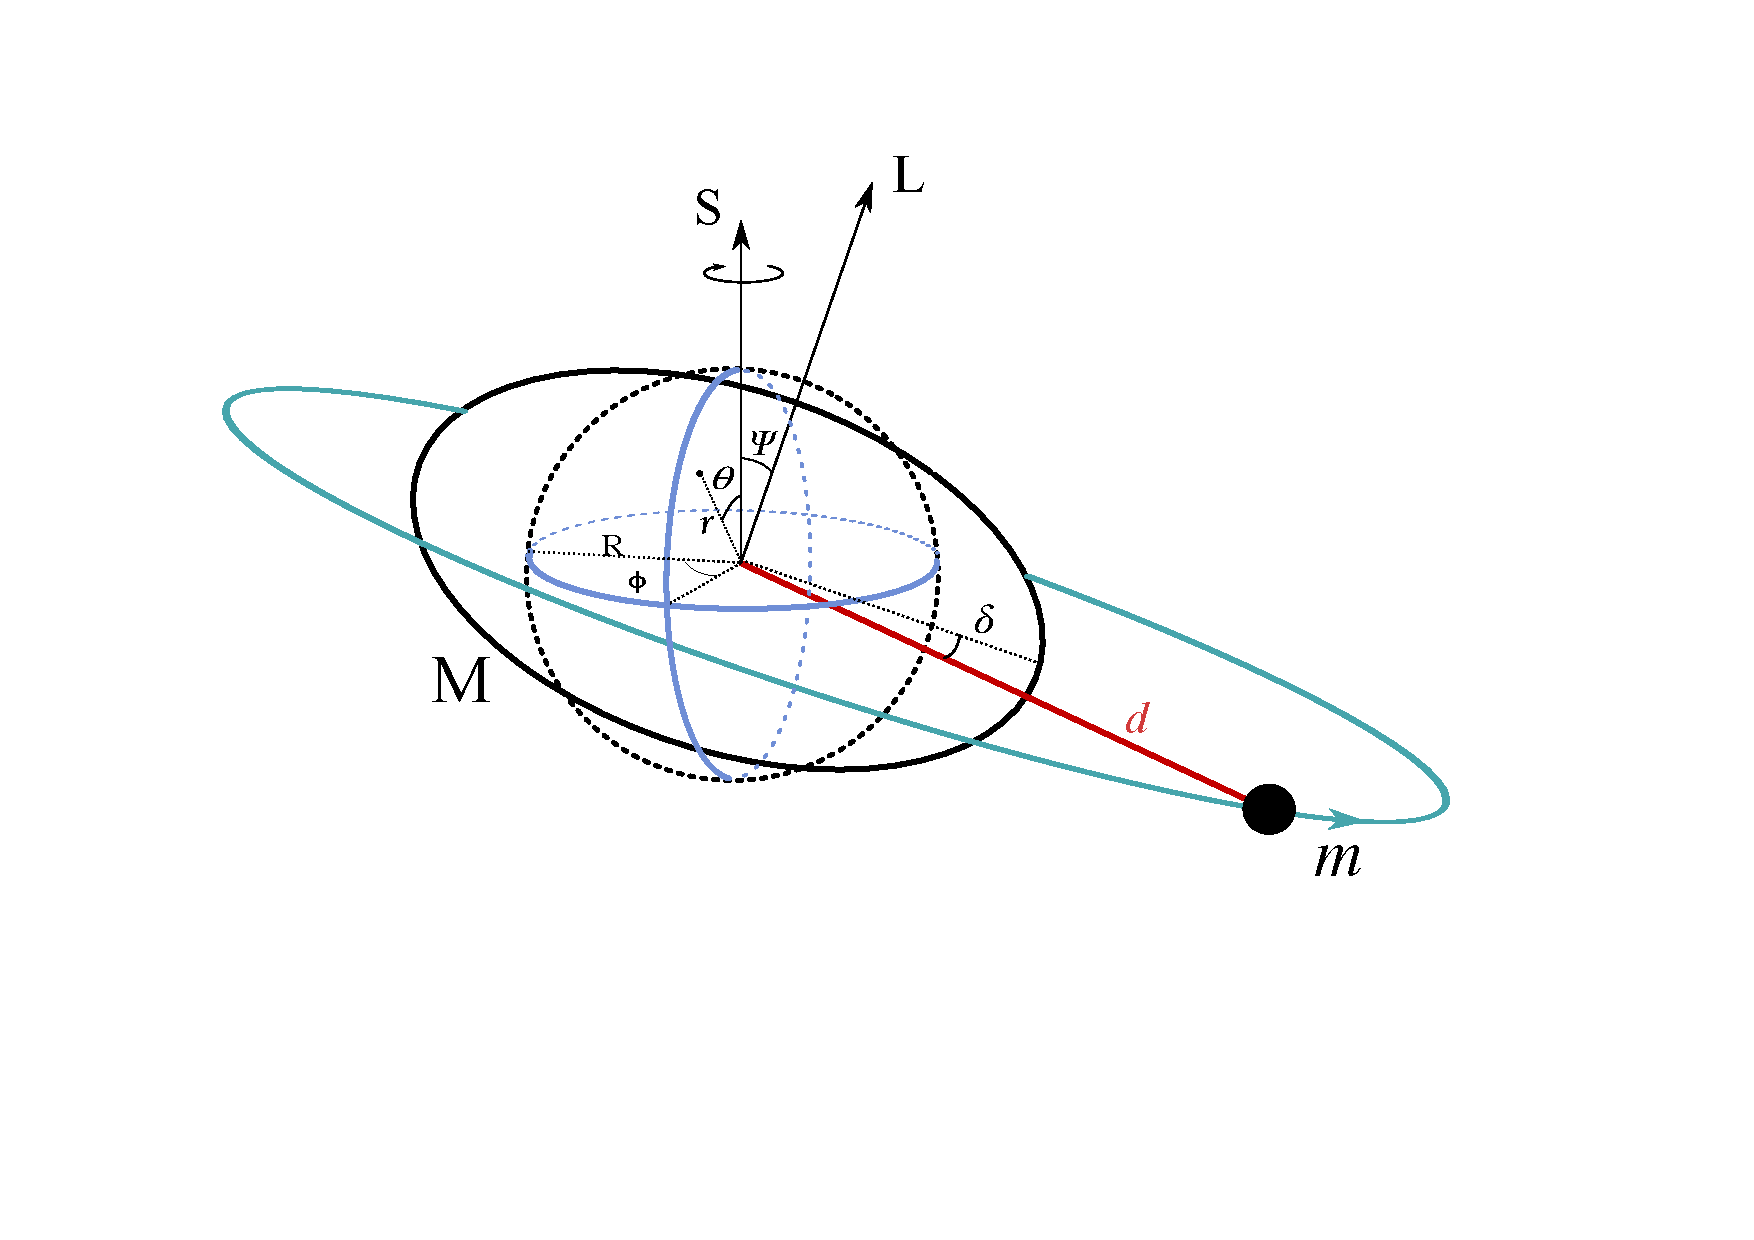
\includegraphics[width=1.0\textwidth]{figures/chapter4/fig4_tides.pdf}
\caption{引力潮汐形变示意图,其中 ($r,\,\theta,\,\phi$) 是以中心天体赤道为基准面的球坐标参考系。$L,\,S$ 分别为扰动体 $m$ 的轨道角动量与潮汐形变体 $M$ 的自转角动量。为了显示,此图的潮汐鼓包被大大地夸张了,并且没有考虑 $M$ 自转产生的鼓包。}
\label{fig:tideillu}
\end{figure}

在上面描述的基础上,如果将潮汐展开精确到二阶($l=2$),并且取角向模数$m,n = 0 $,
便可得到最常用的平衡潮汐(equilibrium tide)模型的近似解。此时形变天体可以用常数滞
后角度(constant phase lag)或滞后时间来参数化描述复杂的潮汐模型:

\begin{equation} \label{eq:eqtide}
Q^{-1}=\frac{1}{2\pi E_0} \oint \big( -\frac{\tif{d} E}{\tif{d} t}\big)\,\tif{d} t = \tan 2\delta \ ,
\end{equation} %\myequation{平衡潮汐模型下的 $Q$ 参数}

Goldreich 和 Soter 于 1966 年将上述模型用在计算太阳系内行星的潮汐耗散率中
\cite{Goldreich1966},同样的理论也用在近距离双星潮汐演化中\cite{Hut1981,Zahn1977}。
对于系外行星而言,HJs 的产生和演化包括两个过程:行星的轨道圆化(circularization)
以及两个天体的轨道自转同步过程(synchronization)。其中每个过程恒星与行星的物质
组成以及内部结构都会影响能量耗散和角动量交换效率,在弱摩擦假设下的平衡潮汐模型
则采用 $Love$ 数 $k_2$ 来描述不同的物质耗散结构。


\section{Rossiter-McLaughlin 效应} \label{sec:rmeffect}

\begin{figure}[b!]
\centering
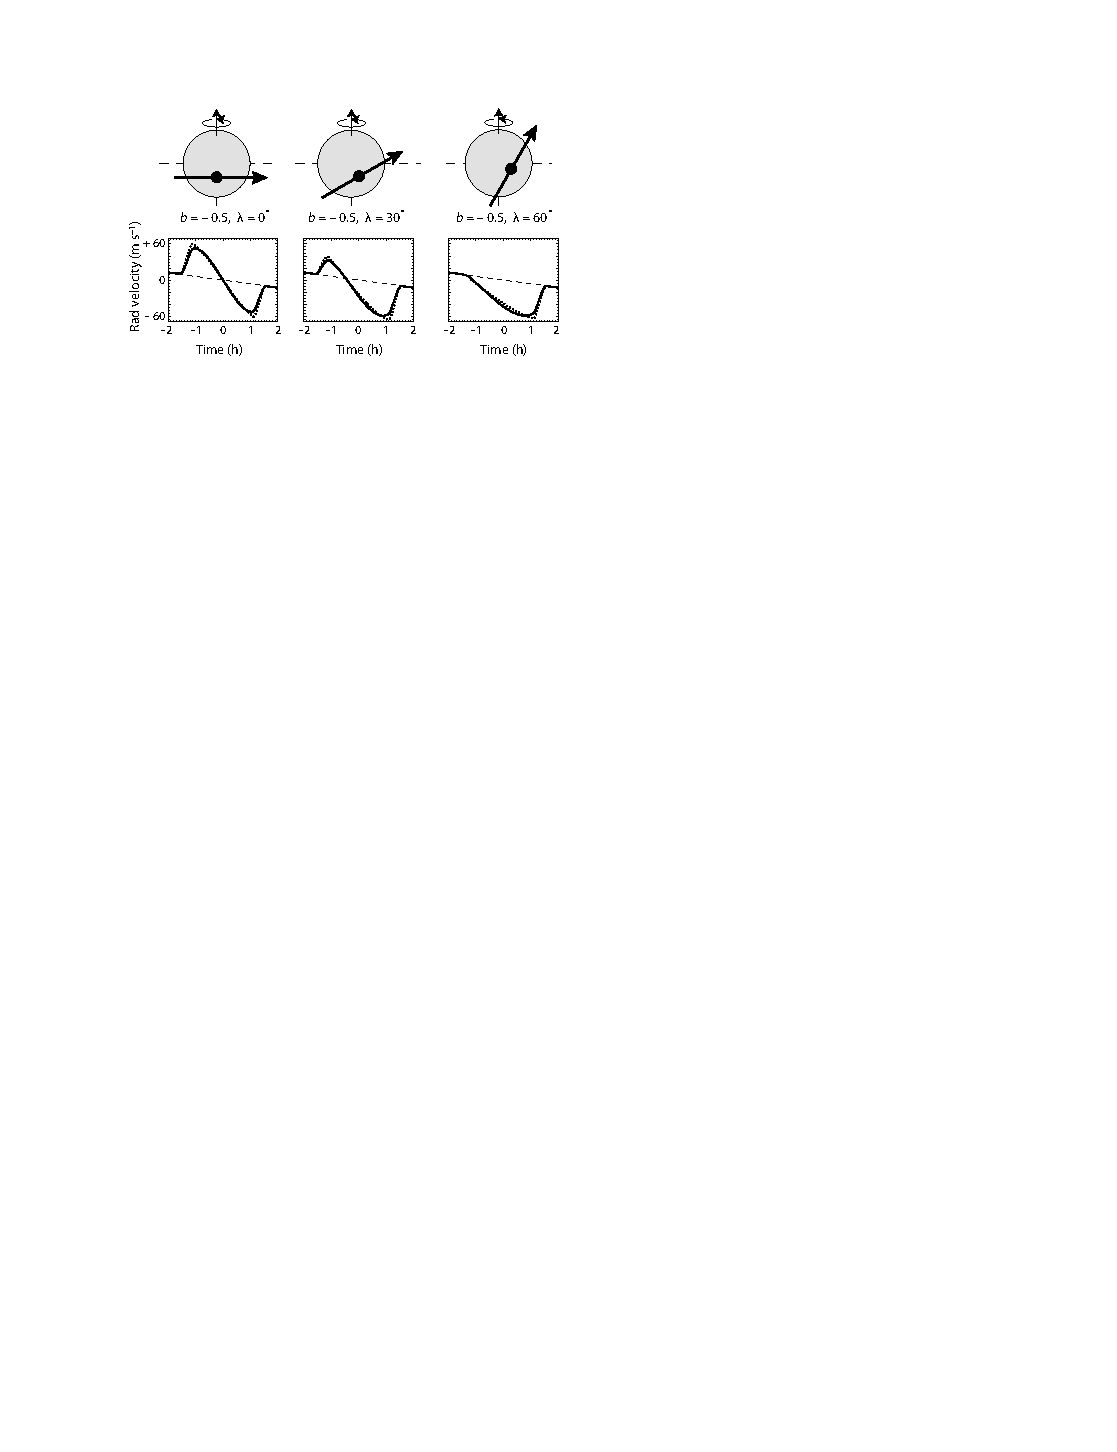
\includegraphics[width=1.0\textwidth]{figures/chapter4/fig5_RMsim.pdf}
\caption[系外行星 Rossiter-McLaughlin 效应示意图。由于行星在凌星过程中遮挡主星的部分区域从而导致主星红移与蓝移的相应部分减小,图中不同的自转---公转倾角以及影响因子均会影响到 RM 效应的视向速度曲线波动轮廓,本图版权 Gaudi/Winn。]{系外行星 Rossiter-McLaughlin 效应示意图。由于行星在凌星过程中遮挡主星的部分区域从而导致主星红移与蓝移的相应部分减小,图中不同的自转---公转倾角以及影响因子均会影响到 RM 效应的视向速度曲线波动轮廓,本图骄傲地取自文献\citen{Gaudi2007}。}
\label{fig:rmsim}
\end{figure}

Rossiter-McLaughlin 效应(RM 效应)最早可能是被 Holt 于 1893 年预言并在双星中观测
证实\cite{Holt1893}。后来 Rossiter 与 McLaughlin 分别详细描述了此过程,并且常常被引
用为 RM 效应\cite{Rossiter1924,McLaughlin1924}。在原理上如果一个天体遮挡住另一天
体,那么背景天体的光谱的视向速度的蓝移与红移部分会分别被遮挡,从而造成视向速度在
掩食内有如下振幅的波动:

\begin{equation} \label{eq:rvdvofrm}
\Delta V_\tif{RM} = (R_\tif{p} / R_\tif{s})^2 \sqrt{(1-b^2)} \, v\sin i
\end{equation} %\myequation{RM 效应的视向速度波动振幅}
其中 $(R_\tif{p} / R_\tif{s})^2$ 约为凌星深度,$b$ 为凌星最大时刻两天体之间的距离影响
因子,$v\sin i$ 为主星的空间投影自转速度。图 \ref{fig:rmsim} 所示为不同的 $b$ 与 
$\lambda$ 参数下恒星视向速度的理论波动,$\lambda$ 在系外行星领域被称作投影行星
轨道法向与恒星自转轴夹角(后文统称自转---公转夹角),为观测测量可拟合量。前文
提到的 $\Psi$ 则为真实的自转--公转夹角,并且本文定义 $0 \leq |\Psi | < 90^\circ$ 为
顺行(prograde)轨道,$90^\circ \leq |\Psi | < 180^\circ $ 则为逆行(retrograde)轨道。


系外行星第一颗被观测到 RM 效应的是 HD209458 系统\cite{Queloz2000},后来陆续有一
大批 HJs 的凌星内 RM 效应被探测到,比如其中非常精确的例子 --- HD 189733(如图 
\ref{fig:rmhd189733}  所示)。在数量稀少的 HJs 系统中,大批量地测量 RM 效应对于研究
其演化过程具有非常重要的作用(将被讨论于下文)。


\afterpage{
\begin{figure}[t!]
\centering
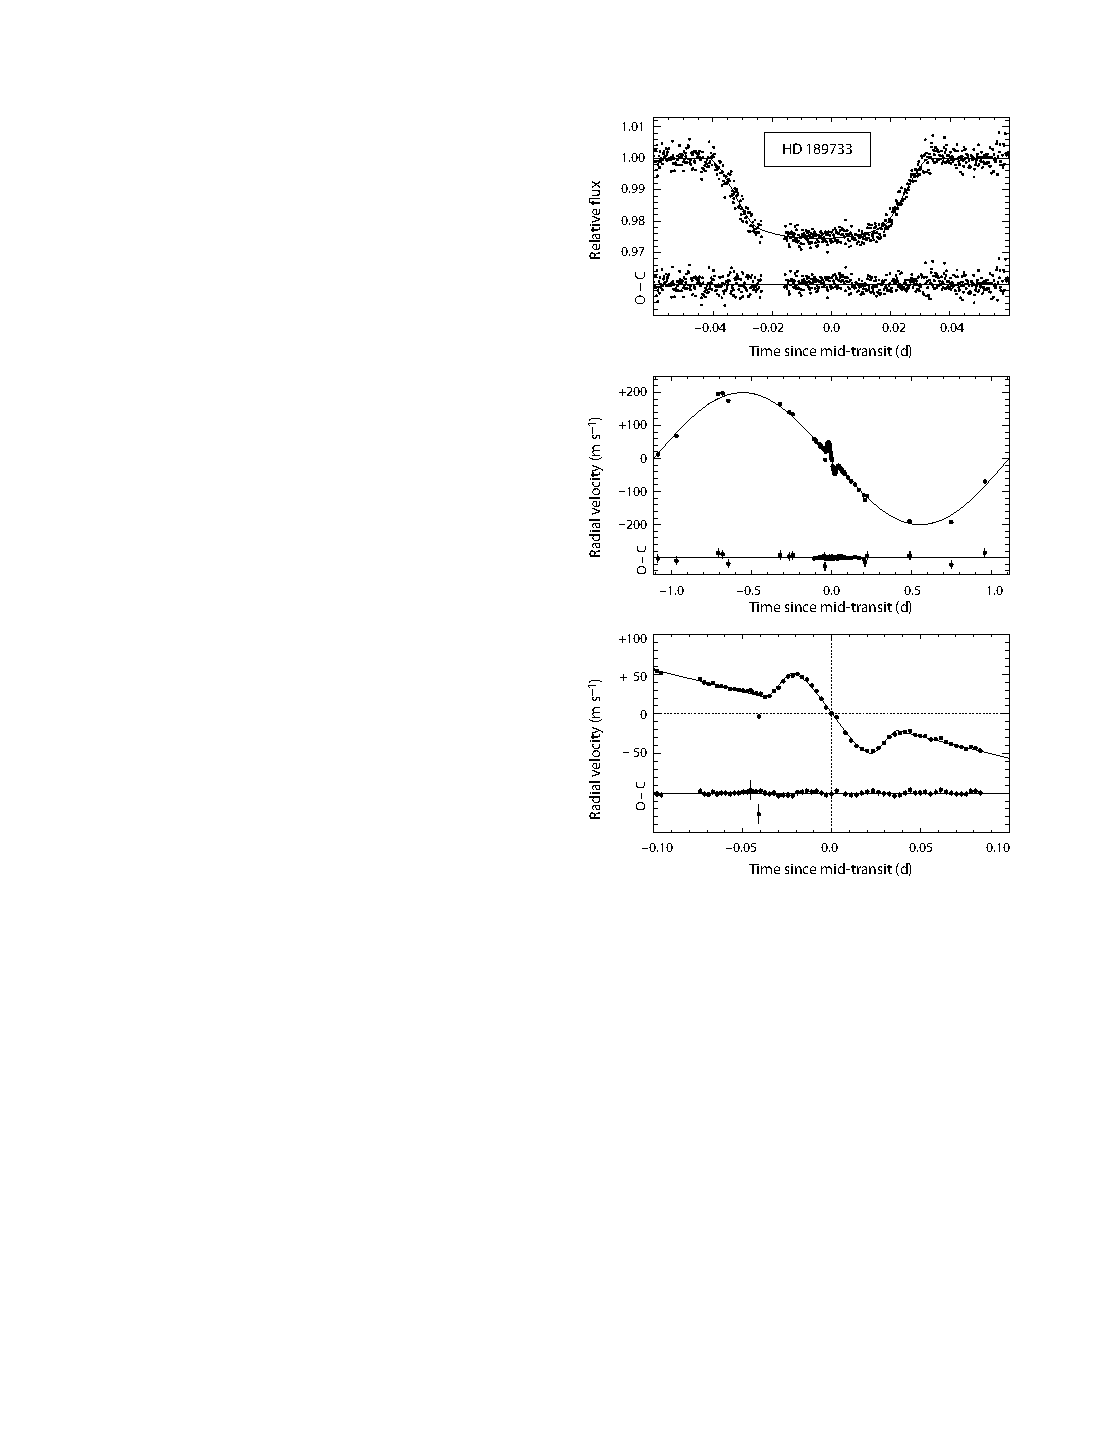
\includegraphics[height=0.90\textheight]{figures/chapter4/fig6_RMHD189733.pdf}
\caption[HD 189733 行星系统凌星内观测到的 RM 效应。上栏为凌星光变曲线,中栏为系统的 RV 曲线周期叠加图,而下栏则为凌星时刻内的 RM 效应,该图版权 Winn 等。]{HD 189733 行星系统凌星内观测到的 RM 效应。上栏为凌星光变曲线,中栏为系统的 RV 曲线周期叠加图,而下栏则为凌星时刻内的 RM 效应,该图取自文献 \citen{Winn2006}。}
\label{fig:rmhd189733} 
\end{figure}
}


\section{热木星的自转轨道倾角}   

在已发现的约 370 颗 HJs 系统中,大约有 100 颗拥有 RM 效应的测量
\footnote{\url{http://www.astro.keele.ac.uk/jkt/tepcat/rossiter.html}}。在 \S \ref{sec:migration} 
中,我们曾提到 HJs 两种主要形成机制气体盘迁移与高偏心率迁移。而这两种形成过程能够产
生截然不同的自转---公转夹角分布。对于传统的盘迁移模型,行星的轨道处于盘的平面内,而
主星的自转轴向量 $\bm{S} $ 被认为和它们的星周盘相互平行,因而 $\Psi$ 角应该比较小。当
然,在一些特殊情况下 $\Psi$ 也可能被激发,比如:恒星形成后期湍动分子云的内流导致盘平
面改变\cite{Bate2010}、磁场---星周盘作用\cite{Lai2011}以及伴星的扰动\cite{Lai2014}。在绝大
部分情况下 $\Psi$ 值应当比较小。相比之下,高偏心率迁移理论(如 Lidov-Kozai 效应)中,
由于伴星的扰动,类木星的轨道倾角则会与偏心率一共大幅度震荡。这样 $\Psi$ 的期望值则应
该在 $[0^\circ,\,180^\circ]$ 之间随机分布。

随着越来越多 HJs 的 RM 效应被探测到,这两种理论也看似总算得以被区分开。Winn 等人于 2011 
年发表了一篇对凌星 HJ 系统 RM 效应统计结果显示:类太阳恒星(GKM Type,$T_\tif{eff} \lesssim 
6250 $ K)周围测量得到的 $\lambda \sim 0$。与之对应的,在偏热 F 型主星($T_\tif{eff} \gtrsim 
6250 $ K) 行星系统中,观测到的 HJs 轨道---自转投影倾角 $\lambda$ 在 0 到 $\pi$ 之间几乎均
匀分布,甚至还包括一些逆行的轨道(文献 \citen{Winn2010},另参见图 \ref{fig:hjobliq})。Albrecht 
随后便给出解释:由于有效温度较低的恒星拥有最外表的对流层,因而它们的潮汐因子 $Q$ 较小,因
此能有效的降低 $\Psi$ 角\cite{Albrecht2012},当然前提便是初始的 $\Psi$ 角随机分布(也因此说明
HJs 更倾向于通过高偏心率迁移模型形成)。

而对于 Albrecht 等使用的潮汐模型,正如前文(\S \ref{sec:tidal})所提到的,其中 $Q$ 值的引入是
一个参数化的模型。这样的模型依赖于类太阳恒星内部对流包层的「混合长」湍动粘滞理论,是通过
不同星团中双星的圆化时标来估算得出\cite{Zahn1977,Mathieu1994},因而模型对类太阳的潮汐耗散
率会由于对流层的存在而被显著增大(中等质量恒星的外表则为辐射包层)。在这样的平衡潮汐模型
下,假设潮汐鼓包处于平衡态之内,那么 $\Psi$ 以及 $\Omega_\tif{s}$ 将会以相同的速率演化。而潮
汐演化通常引来行星半长径 $a$ 的演化。对于低质量恒星,其周围的木星公转轨道角速度 $n=2\pi/P 
> \Omega_\tif{s}$,因此木星将会转移角动量给主星,因而轨道会内迁。在 Albrecht 等人的理论中,
此轨道内迁速度必须得慢于 $\Psi$ 减小的速度。对于有效温度稍高的主星($\Omega_\tif{s} > n$),
它们的角动量会转移给热木星,因此这类 HJs 必须在从距离主星半径($R_\tif{s}$)更近的位置演化
\cite{Rogers2013}。

\begin{figure}[t!]
\centering
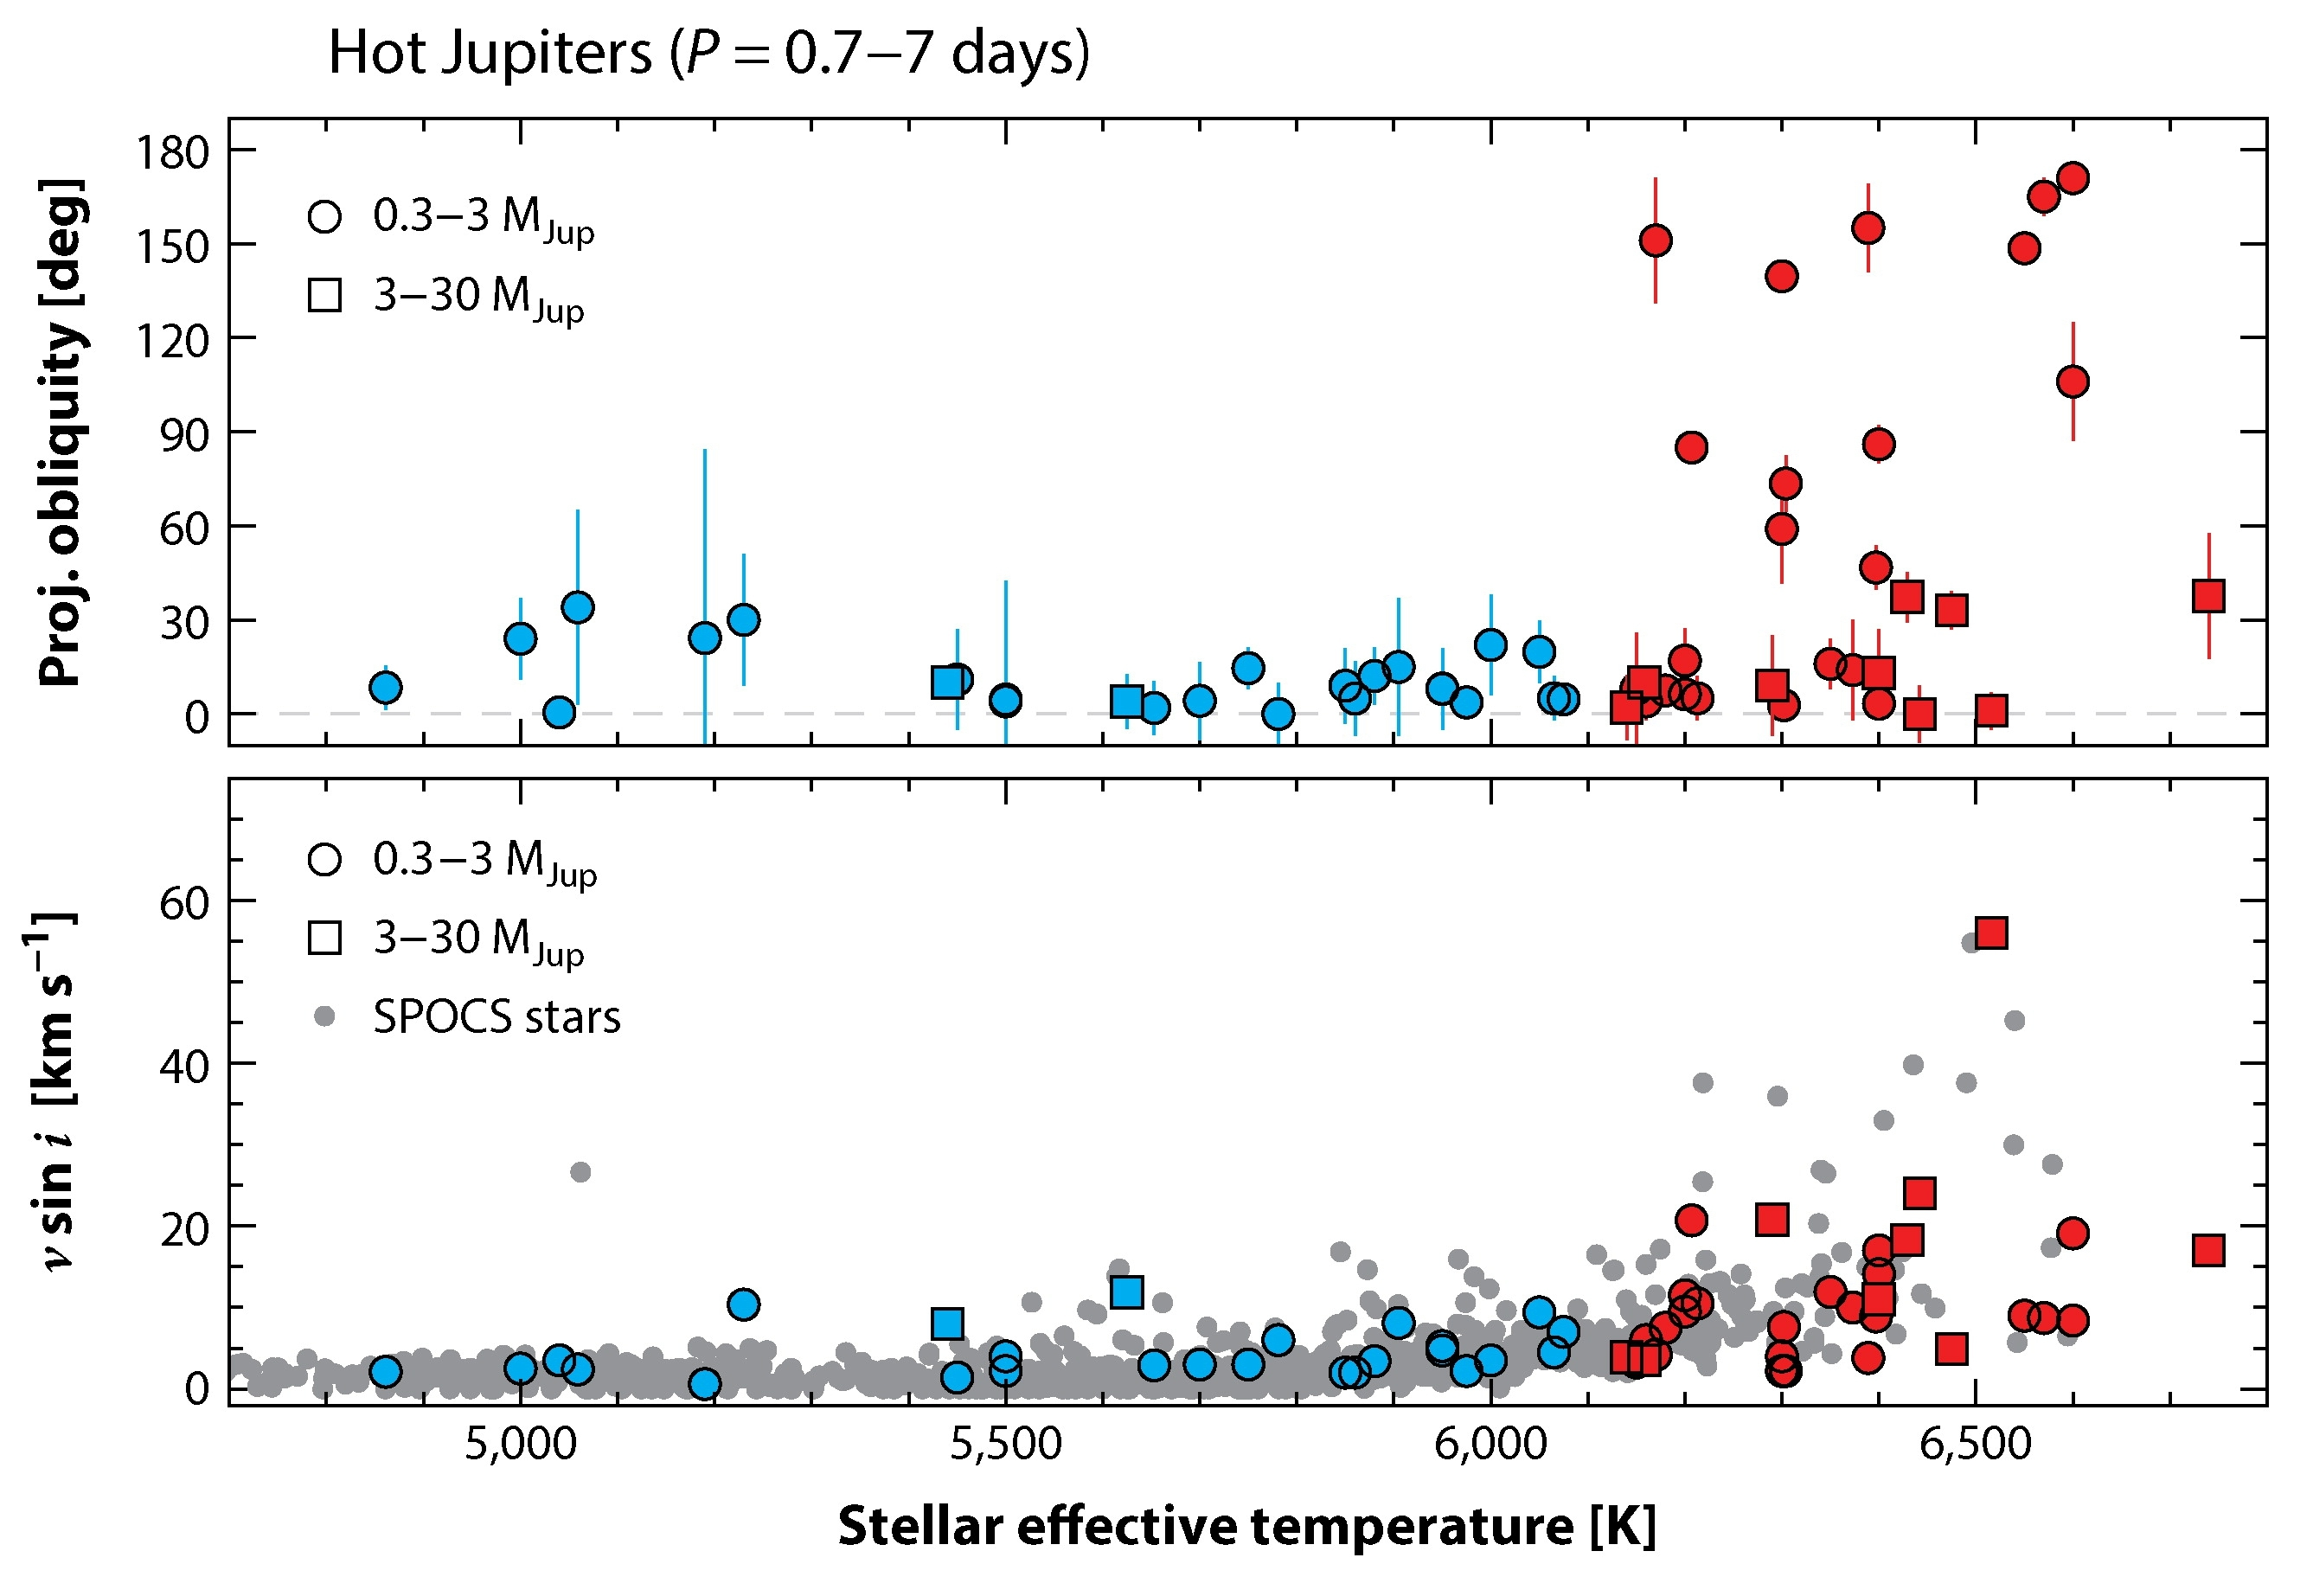
\includegraphics[width=1.0\textwidth]{figures/chapter4/fig7_hjobliq.jpeg}
\caption[上栏为 HJs 的主星有效温度与投影自转---公转夹角 $\lambda$ 的统计图,下栏为恒星的投影自转速度与有效温度的统计关系。可以看到有效温度较高的恒星明显拥有较大的自转速度,而这部分恒星正好对应几乎均匀分布的 $\lambda$ 值。图片版权 Winn 和 Fabrycky。]{上栏为 HJs 的主星有效温度与投影自转---公转夹角 $\lambda$ 的统计图,下栏为恒星的投影自转速度与有效温度的统计关系。可以看到有效温度较高的恒星明显拥有较大的自转速度,而这部分恒星正好对应几乎均匀分布的 $\lambda$ 值。图片取自文献 \citen{WinnFabrycky2015}}
\label{fig:hjobliq}
\end{figure}

为了解决这里的自转公转的共面演化与轨道退化时标问题,一些不同的理论也被相应地被提出,包括:
\textbf{(1)} Lai 建议将动力学潮汐(dynamical tide)模型将 $\Psi$ 的演化与平衡潮汐的演化区分开
\cite{Lai2012},也即除了处于流体静力学的平衡潮汐以外,内引力(internal gravity)与惯性波(inertial 
wave)同样可以在稍热恒星的内部被激发\cite{Ogilvie2004,Ogilvie2007,Ogilvie2014}。此类机制的潮汐
响应频率与振幅和热恒星内部的结构以及耗散机制有关\cite{Ogilvie2007}。由于潮汐扰动频率不同,因而
对应于轨道圆化、轨旋同步以及自转---公转同步演化的等效 $Q$ 值可能会大不相同。甚至在某些 
$\Omega_\tif{s}/n$ 的特定取值下,$\Psi$ 可在轨道几乎不变的同时衰减为零\cite{Lai2012},类似的演化
会将 $\Psi$ 的分布集中在 0,$90^\circ$ 与 $180^\circ$ 三个值附近\cite{Rogers2013,Xue2014},然而
观测却没有相关的证据来符合此分布。\textbf{(2)} Dawson 于 2014 年提出类太阳恒星的磁阻尼
(magnetic breaking)效应\cite{Kraft1967}会使得它们的自转角动量大大减小,因而 HJs 只需要很小部
分的角动量即可使得恒星的自转与 HJs 公转指向一致。这样 HJs 的轨道半长径不会在 $\Psi$ 被减小至
零之前就小于恒星的半径(被主星吞噬)\cite{Dawson2014}。


当然,前文我们提到高偏心率迁移并不是唯一能解决观测到的自转---轨道指向不一致的问题,但是这些
机制中的 HJs 虽然可以通过盘的迁移达到主星附近几天周期的轨道,但是若想解释两种恒星中 $\Psi$ 值
的差异还是得需要引入潮汐。在这些理论中,唯一不依赖于潮汐耗散率的解释便是 Rogers 于 2012 年提
出的理论:温度较高的恒星自转轴会由于内部重力波(internal gravity wave,简称 IGW)而被重新指向。
由于中等质量的恒星外层为辐射包层,内核则对流的,而 IGWs 则能够在对流辐射层分界面上产生并且向
外部传播截至于恒星的确表面并改变恒星外层的转动方向\cite{Rogers2012,Rogers2015}。在慢速自转的恒
星中,此机制可以在观测中产生明显的非零 $\Psi$ 值(即使初始值为零),而同样在低质量类太阳恒星
中,此机制却不能被激发,因而可以解释观测中的两种恒星的 $\Psi$ 统计分布。


\subsection{统计数据筛选}

\begin{figure}[t]
\centering
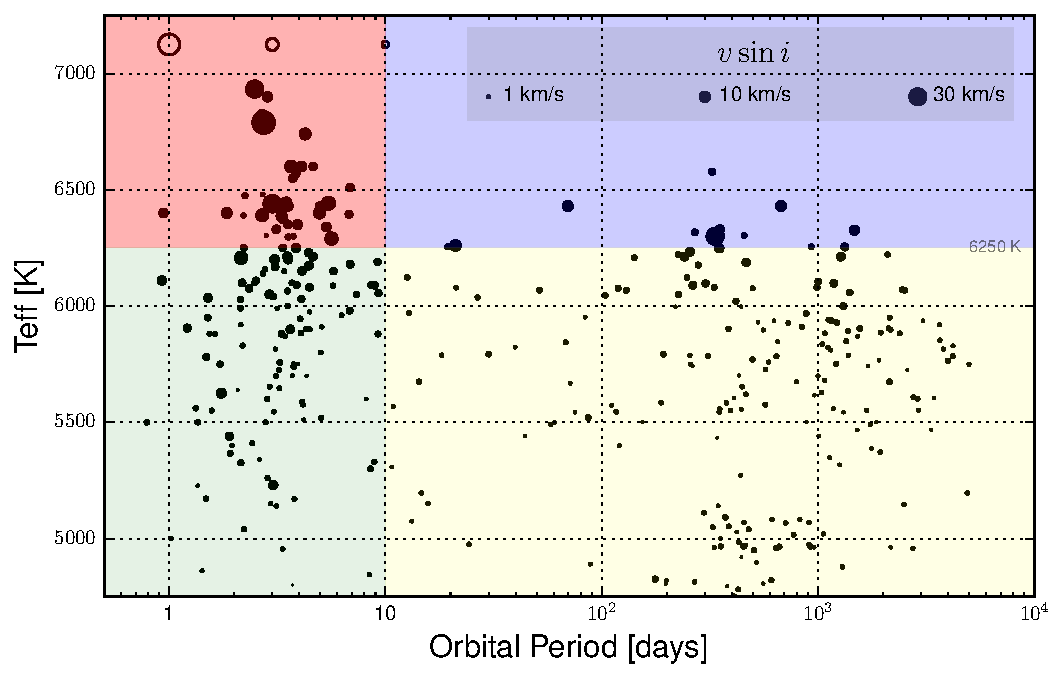
\includegraphics[width=1.0\textwidth]{figures/chapter4/fig8_perteff.pdf}
\caption{已知系外气巨星的轨道周期与主星有效温度分布图,点的大小正比于主星投影自转速度的对数。在此图的左上角分别标注了对应行星周期 $P$ 为 1、3、10 天 处,一个太阳质量恒星的同步自转速度 $V_\tif{s} $(分别为 50.6、16.8、5.0 km/s) 。从图中可以看到大部分类太阳系统拥有 $\Omega_\tif{s} < n$,除了少部分较热恒星周围行星轨道角速度小于恒星自转速度,此图中不同温度的恒星自转速度与行星周期的相关性应该为观测选择效应。}
\label{fig:perteff}
\end{figure}

为了检验已有的相关理论,本文利用本章开始所整合的 HJs 数据,并且综合 RM 效应,通过以下条件筛
选现有数据以提供给后文分析:

\begin{enumerate}
\item 每个行星系统必须包括行星质量($M_\tif{p}$)或最小行星质量($M_\tif{p} \sin i$)、轨道周期
($P$)或轨道半长径($a$)这两类观测量。
\item 由于超级地球的质量并不足以通过潮汐来改变主星的自转性质,因此我们将样本限制在大于土星质
量的系外行星。
\item 该行星系统的宿主恒星必须有较好的质量 $M_\tif{s}$、半径 $R_\tif{s}$、有效温度 $T_\tif{eff}$ 以及
投影自转速度 $v \sin i$ 的测量。
\item 每个上述物理量 $\xi$ 需要拥有小于一半的测量误差,即 $\Delta \xi  \leq 0.5 \, \xi$。
\end{enumerate}

以上挑选后的数据在图 \ref{fig:perteff} 中被分成四种不同的类别:较热恒星($T_\tif{eff} > 6250 $ K)、
较冷类太阳恒星($T_\tif{eff} < 6250 $ K)分别被短周期($P < 10 $ 天)、长周期($P >10 $ 天)的
气巨行星环绕。本文将这四种不同类型的行星数目以及平均恒星自转速度统计在列表 \ref{tbl:stat} 中,
它们分别为高温度短周期(HS)、高温度长周期(HL)低温度短周期(CS)与低温度长周期(CL)。
热恒星在长周期上观测到的行星数目明显偏少是由于 RV 观测的选择效应导致的,并且 RV 以及凌星
都偏向于观测自转偏慢恒星周围的行星。在图中,热恒星自转速度明显要快于冷恒星的自转($v\sin i$ 
--- $T_\tif{eff}$)则是因为有低质量恒星的星风磁阻尼效应\cite{Kraft1967}。

{\renewcommand{\arraystretch}{1.3}
\begin{table}[t]
\centering
\caption{按照主星性质分类下,不同行星系统的统计数据}
\label{tbl:stat}
\begin{tabularx}{0.9\textwidth}{@{\extracolsep{\fill}}lcc}
\toprule
  &  Mean $v \sin i $ [km/s]  & Number of systems \\ \midrule 
HS & 16.7       & 38                \\ 
HL & 11.5       & 12                 \\ 
CS & 4.5        & 129               \\ 
CL & 2.9        & 196                \\ \bottomrule
\end{tabularx}
\end{table}
}

\subsection{行星公转---恒星自转潮汐演化} \label{sec:obliquityevo}

对于热木星系统而言,系统的总角动量主要是由主星的自转角动量与行星轨道角动量组成的(行
星自己的自转角动量与主星绕质心公转的角动量均小两个量级以上,因此可以忽略)。主星的自
转角动量为

\begin{equation} \label{eq:spinam}
J_{*,\,\tif{spin}} \equiv S = \gamma_\tif{s} M_\tif{s} R_\tif{s}^2 \Omega_\tif{s} \ ,
\end{equation} %\myequation{恒星自转角动量}
其中 $\gamma_\tif{s}$ 为恒星转动惯量系数。行星的轨道角动量则为 $L = M_\tif{p}na^2$(参见
公式 \ref{eq:2bam})。在潮汐力矩的作用下,整个系统的总角动量($S+L$)守恒,因此可以得
到恒星的自转角动量变化率与行星公转角动量变化率满足关系式 $\dot{J} = \dot{S}$。

不失一般性,取 $\Psi$ 为恒星自转与行星公转法向任意夹角,行星对主星的平衡潮作用将会使得
行星的轨道半长径、主星的自转与行星轨道法向角度以及主星的自转速度有如下变化

\begin{subequations} \label{eq:tidalevo}
\setlength{\jot}{10pt}
\begin{align}
   \dot{\Psi} &= - \frac{L\sin \Psi f_\Psi(\Psi)}{2S_{\tau_e}}     \label{eq:obevo} \\
    \frac{\dot{a}}{a} &= - \frac{f_a(\Psi)}{\tau_e}   \label{eq:smaevo}  \\
    \frac{\dot{\Omega}}{\Omega} & = \frac{Lf_\Omega(\Psi)}{2S_{\tau_e}} \label{eq:spinevo}
\end{align}
\end{subequations} %\myequation{潮汐对行星轨道以及恒星自转的影响}
其中 $f_\Psi(\Psi) = 1 - (\Omega_\tif{s}/2n)(\cos\Psi - S/L)$,$f_a(\Psi) = 1 - (\Omega_\tif{s}/n)\cos\Psi$,
$f_\Omega(\Psi) = \cos\Psi - (\Omega_\tif{s}/2n)(1+ \cos^2\Psi)$(文献 \citen{Goldreich1966,
Eggleton1998,Ogilvie2004})。典型的潮汐演化时标则为:

\begin{equation} \label{eq:taue}
\tau_e \equiv \left( {Q_\tif{s} \over 3 k_2} \right) \left( {M_\tif{s} \over M_\tif{p}}\right)
\left( {a \over R_\tif{s}}\right)^5 \left( {P \over 2 \pi} \right) 
\end{equation} %\myequation{典型的潮汐演化时标}

在方程 \label{eq:taue} 中,一般会采用 Goldreich 与 Stoer 的潮汐参数记号 $Q_\tif{s}^\prime \equiv 3 
Q_\tif{s}/2k_2$,其中 $k_2 =1.5/(1+{\tilde \mu})$,且 ${\tilde \mu} = 19 \mu/(2 \rho_\tif{s} 
g_\tif{s} R_\tif{s})$ 为等效刚性系数, $\mu$,$\rho_\tif{s}$ 和 $g_\tif{s}$ 则分别为主星的刚性系数、
密度以及表面重力。

对于中等小大的 $\Psi$,可有 $f_\Psi \simeq 1 - (\Omega/2n) (1-S/L)$,$f_a \simeq f_\Omega \simeq 1
 - \Omega/n$(精确到 $\Psi$ 的二阶),从而有
 
\begin{subequations} \label{eq:ttimescale}
\setlength{\jot}{10pt}
\begin{align}
    \tau_a &\simeq - \frac{L}{2S}\tau_\Omega \simeq \frac{L}{2S} \frac{f_\Psi}{f_a} \tau_\Psi \\
    \tau_\Psi &\simeq -\frac{f_\Omega}{f_\Omega} \tau_\Omega 
\end{align}
\end{subequations} %\myequation{潮汐对行星轨道以及恒星自转的影响}
其中我们定义 $\tau_a \equiv a /{\dot a}$,  $\tau_\Omega \equiv \Omega / {\dot \Omega}_{\tif{s, t}}$, 
$\tau_\Psi \equiv \Psi / {\dot \Psi}$ 为典型的行星轨道、恒星自转以及自转---公转夹角演化时标。

在本文内,我们考虑了将不同系统的 $Q_\tif{s}^\prime$ 值,因为该参数依赖于何种湍动粘滞机制\cite{
Zahn1977,Goldreich1989,Penev2007}、内部结构\cite{Terquem1998,Goodman2009}以及自转速率
\cite{Ogilvie2007,Barker2009}密切相关。在弱摩擦近似下的平衡潮汐模型下,$Q_\tif{s}^\prime$ 与
潮汐强迫震动频率无关,因而在处理 $\dot{a}$,$\dot{\Omega}_\tif{s}$,$\dot{\varPsi}$ 时并不需要
加以区分,因而 $\tau_a / \tau_\Psi$ 也并依赖于$Q_\tif{s}^\prime$ 值的选择。

观测中,大部分围绕低质量低温慢速自转类太阳恒星的 HJs 都满足 $n>\Omega_\tif{s}$,也即它们的
公转同步自转半长径 $a_\tif{cr} = (GM_\tif{s}/\Omega_\tif{s}^2)^{1/3} = (GM_\tif{s}R_\tif{s}^2/V_\tif{s}^2)^{1/3}$,
加上符号后,$\tau_a (<0)$,$\tau_\Omega (>0)$ 以及$\tau_\Psi (<0)$ 分别对应于轨道收缩,恒星自
转加速和轨道自转同向。在这样的极限下 $f_a$, $f_\Omega$ and $f_\Psi$ 均趋近于单位一,与之对应
的角动量比值 $L/2S$ 可从小于一取值到大于一。

进一步延伸公式 \ref{eq:ttimescale} 后,可以得到对于快速自转的主星($L<2S$)周围的行星轨道会
在自转---公转夹角演化前便显著收缩($\tau_a < \tau_{\Omega},\tau_\tif{s}$)。若要使得这部分在它
如今的轨道上存活,就必须要求半长径演化的时标 $\tau_a$ 能够大于或者与恒星的年龄相当($\tau_
\tif{s}\sim \tau_\odot$ 其中 $\tau_\odot =4.6$ Gyr 为太阳如今的年龄),也即

\begin{equation} \label{eq:qorbit} 
Q_\tif{s}^\prime > Q_{\rm orbit} \equiv {9 \tau_\tif{s} \over 2} 
{M_\tif{p} \over M_\tif{s}}  \left( {G M_\tif{s} \over R_\tif{s}^3} \right)^{1/2}
\left({R_\tif{s} \over a} \right)^{13/2}.
\end{equation}  %\myequation{行星轨道演化所需求的平衡潮参数}
其中我们引入 $Q_{\rm orbit}$ 来指示过去行星轨道的平衡潮演化参数。这里我们将前文提到的恒星内部
的耗散参数 $Q_\tif{s}^\prime $ 全部记成 $Q$ 以示美观。

然而另一方面,对于缓慢自转的恒星($L>2S$),情况则会有所不同。这部分恒星的自转轴---行星的轨道
法向夹角 $\Psi$ 会有显著的演化,尽管行星轨道并未发生变化($\tau_a >\tau_{\Omega},\tau_{\tif{s}}$)。
对于这部分系统而言,改变主星 $\Omega_\tif{s}$ 或者 $\Psi$ 则仅需要轨道少量变化即可。因而只有满足
$\tau_\tif{s}>\tau_\Psi \simeq 2S \tau_e/L$ 的系统才能使得恒星自转与自转---轨道夹角有显著的演化(参
见公式 \ref{eq:tidalevo}),也即对应于

\begin{equation}  \label{eq:qspin}
Q_\tif{s}^\prime < Q_{\rm spin} \equiv {9 G M_\tif{s} \tau_\tif{s} 
\over 4 \gamma_\tif{s} R_\tif{s}^2 V_\tif{s}} 
\left( {M_\tif{p} \over M_\tif{s}} \right)^2 
\left({R_\tif{s} \over a} \right)^{6}.
\end{equation} %\myequation{恒星自转演化所需求的平衡潮参数}
这里的 $Q_{\rm spin} $ 为过去主星自转(以及自转---公转夹角)的平衡潮演化参数,其中公式 \ref{eq:qorbit} 
与公式 \ref{eq:qspin} 之间满足关系 $Q_{\rm spin} = L/2S Q_{\rm orbit}$。

对于满足 $L< 2S$ 的系统,它们不可能在 HJs 的轨道不显著内缩的同时,对主星的自转速度以及自转轴
取向造成可观的该变量。相反当 $L>2S$时,我们便可找到对应的 $Q_\tif{s}^\prime $ 来同时满足公式 
\ref{eq:qorbit} 与公式 \ref{eq:qspin} ,也即 $Q_{\rm orbit} < Q_\tif{s}^\prime < Q_{\rm spin}$。在此范围
内热木星公转法向与主星自转轴方向可被潮汐趋同化。需要说明的是,这里的条件和真实的恒星 $Q$ 值并
不相关。

在这两种情况之间,我们可以计算得到自转---公转的临界值,它定义为 $L=2S $时,主星的临界自转速率

\begin{equation} \label{eq:vc}
V_c \equiv {M_\tif{p} {\sqrt{G M_\tif{s} a}} /( 2 \gamma_\tif{s} m_\tif{s}R_\tif{s}}).
\end{equation} %\myequation{潮汐演化中恒星自转速度的临界取值}

对于在快速旋转恒星($\Omega_\tif{s} > n$)周围的行星,若其轨道半长径满足 $a > a_{cr}$,那么它将会
接受来自恒星的角动量,轨道也将	扩张至当前观测的位置附近。而由于在方程 \ref{eq:taue} 中 $\tau_a 
\propto \tau_e$ 是十分敏感依赖于 $a$ 值的函数,因此公式 \ref{eq:qspin} 能比较好限定当前主星的潮汐参
数 $Q$ 值。下面我们将对中等质量的恒星以及低质量类太阳恒星分别分析统计的结果。

\subsection{中等质量恒星} \label{sec:hotstar}

\begin{figure}[t]
\centering
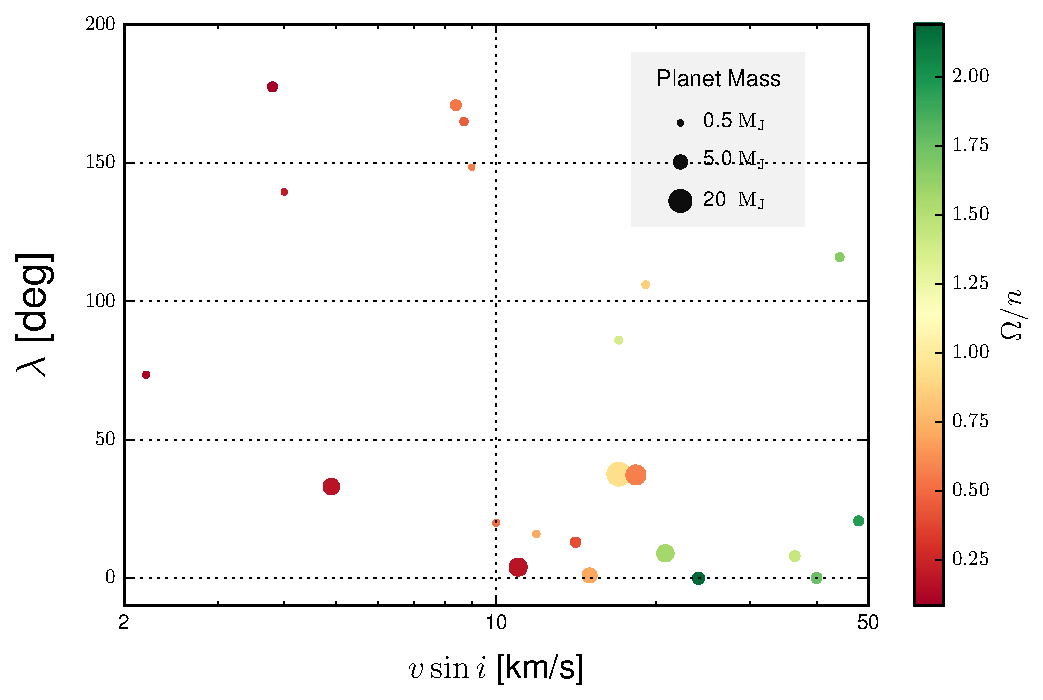
\includegraphics[width=1.0\textwidth]{figures/chapter4/fig9a_hot.pdf}
\caption{所有中等质量恒星周围已知 $\lambda$($\Psi$) 的 HJs 散点图。图中点的大小代表行星的质量 $M_\tif{p}$,颜色则代表 $\Omega/n$。可以看到自转偏慢的恒星反而拥有比较大的 $\lambda$。而且图中至少有七个系统拥有 $\Omega > n$,这代表了这些系统内行星轨道发生了外迁。}
\label{fig:hotobliquity}
\end{figure}


\afterpage{
\begin{figure}[t]
\centering
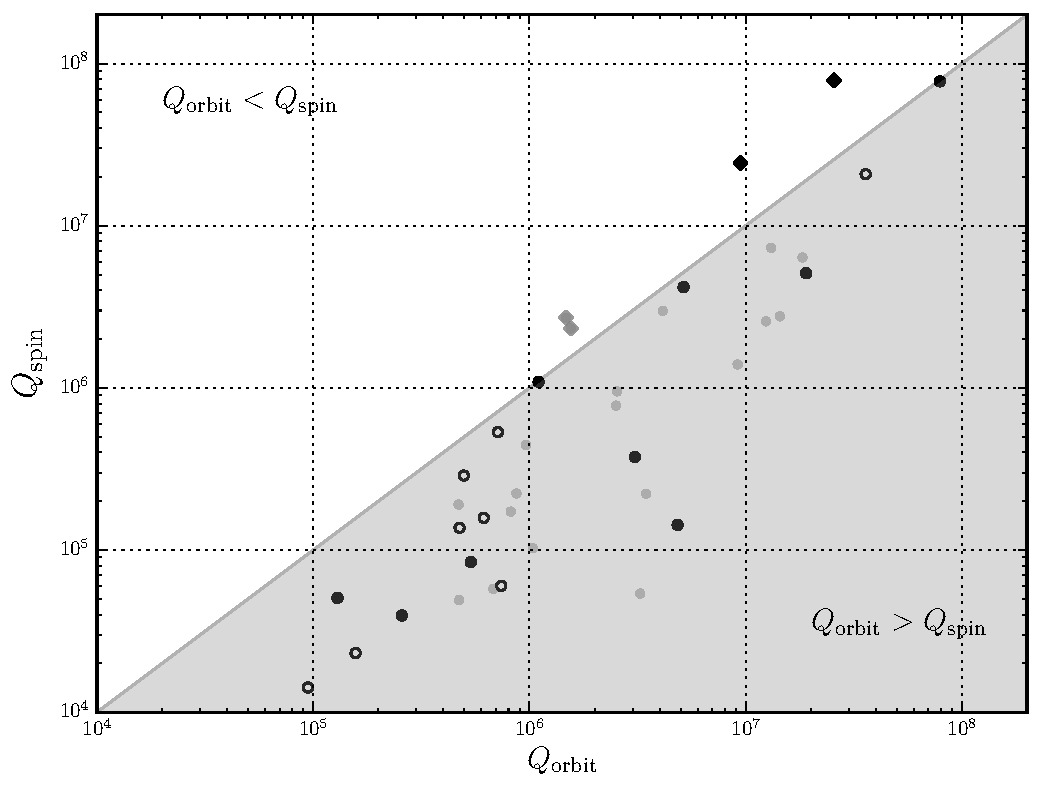
\includegraphics[width=1.0\textwidth]{figures/chapter4/fig9b_hot.pdf}
\caption{根据公式 \ref{eq:qorbit} 与 \ref{eq:qspin} 计算得到的热恒星对应的临界 $Q_\tif{orbit}$ 与 $Q_\tif{spin}$ 值分布图。 黑色的实心圆与空心圆分别代表自转轨道法向吻合($\lambda < 30^\circ$)与不吻合($\lambda > 30^\circ$)的系统,对于 $\Omega_\tif{s} > n$ 的系统则用菱形来表示,灰色的点则表示没有$\lambda$ 的观测数据信息。}
\label{fig:hotqq}
\end{figure}
}

首先我们将如上分析应用至热恒星中,这部分恒星周围不太可能有很强的星风。在图 \ref{fig:hotobliquity} 
中,我们将此类系统中观测到的 HJs 投影 $\Psi$ 角 $\lambda$ 和主星的有效温度分别画在纵轴与横轴上。
在平衡潮汐的模型下,红色的系统($\Omega_\tif{s} < n$)中行星轨道将会收缩,而少数绿色的系统(
$\Omega_\tif{s} > n$)则会膨胀,且这些快速自转系统的 $\Psi$ 值相对较小。与此同时自转---公转高度不
吻合的系统($\Psi$ 值较大)反而和自转偏慢的系统相关。在文献 \citen{Dawson2014} 的描述中,自转偏
慢的恒星拥有较小的角动量,因此这些主星的自转轴应该会更容易受其行星的潮汐作用影响。从这些系统
中发现的自转---公转不一致性和自转速度的反相关性和以往普遍认为的慢速自转恒星更容易手潮汐作用的
影响是不自洽的\cite{Rogers2013,Li2016}。

同样这些系统的  $Q_\tif{orbit}$ 与 $Q_\tif{spin}$ (公式 \ref{eq:qorbit} 和 \ref{eq:qspin})也被对应地画在
图 \ref{fig:hotqq} 中:黑色点 --- $\Psi < 30^\circ$,黑色空心点 --- $\Psi > 30^\circ$ 以及灰色点标注的没有
测量数据的系统。不失一般性,我们采取 $\tau_\tif{s} \sim \tau_\odot = 4 $ Gyr,以及 $\gamma_\tif{s} = 0.2$
不同恒星这些值可那个会有所差别,但是并不会让它们穿越对角线($Q_\tif{orbit} = Q_\tif{spin}$)。

如果潮汐能够在这些系统中起作用的同时行星也不会坠入主星内,那么主星的潮汐值参数 $Q_\tif{s}^\prime$
应该在区间 $Q_\tif{orbit} < Q_\tif{s}^\prime <  Q_\tif{spin}$ 以内。从图中可以明显的看到大部分系统都落在
了灰色区域 $Q_\tif{orbit} >  Q_\tif{spin}$ 内,因而这些系统不能在不显著缩小轨道的同时,通过潮汐作用改
变主星的自转取向(参见章节 \S \ref{sec:obliquityevo})。

也有小部分系统处在 $L> 2S$ 的边界处,这样的系统都是快速自转的系统($\Omega_\tif{s} > n$,菱形的数
据点)。对于这些系统,行星的轨道处于共转半长径以内,过去的潮汐作用只会导致该系统 $L/2S$ 的值增加。
而 $Q$ 也会随着时间的增长而增加(即过去恒星的 $Q$ 值更小),因此过去这些系统的潮汐作用会更强。而
从它们的 $\Psi$ 偏大表示过去更强潮汐作用并没有在它们之中起主导作用。甚至有些系统的潮汐演化时标已经
明显长于主星的年龄(在图 \ref{fig:hotqq} 中 $Q \gtrsim 10^{6-8}$),这也进一步支持了行星与恒星之间的潮
汐作用可能比双星之间的作用弱得多\cite{Ogilvie2007}。


\subsection{类太阳恒星} \label{sec:coolstar}

对于有效温度较低的类太阳主星,它们自转的速度明显小于上文提到的高温恒星(见图 \ref{fig:perteff}),
这是因为此类恒星可通过星风来流失质量与损失原初角动量。这样的效应在观测上则一般引用文献
\citen{Skumanich1972,Soderblom1983} 中的经验公式来定量描述,具体形式如下

\begin{equation} \label{eq:wind}
V_\tif{s} \simeq  V_0 \bigg( \frac{t}{t_0} \bigg)^{-1/2}
\end{equation}
这里的 $t_0$ 与 $V_0$ 在本文分别取为 $\simeq$1 Gyr 与 $\simeq$ 4 km s$^{-1}$。在星风与潮汐的同时
作用下\cite{DobbsDixon2004,Dawson2014},对恒星自转速度影响的总效应则为:$\dot{\Omega}_\tif{s} 
\simeq \dot{\Omega}_\tif{s, t} + \dot{\Omega}_\tif{s, w}$,其中 $\dot{\Omega}_\tif{s, t}$ 为潮汐带来的自转
变化率,$\dot{\Omega}_\tif{s, w}$ 则为星风相应的贡献。利用公式 \ref{eq:wind},我们可以得到 
$\dot{\Omega}_\tif{s, w} = -\Omega_\tif{s}^3 R_\tif{s}^2/2 t_0 V_0^2$。星风作用仅仅体现在减慢恒星的自转
速度上,当自转速度衰减的同时,转速的变化率 $ \dot{\Omega}_\tif{s, t}$ 和 $\dot{\Omega}_\tif{s, w}$ 也一
并减少,直到最终 $ \dot{\Omega}_\tif{s} \approx 0 $。在此情况下,所有的低质量恒星以及其热木星都会
演化至星风与潮汐平衡的状态,也即 $\dot{\Omega}_\tif{s, t} = - \dot{\Omega}_\tif{s, w}$ 或者:

\begin{equation} \label{eq:lmeq}
{V_e \over V_0} \equiv \frac{\Omega_eR_\tif{s}}{V_0} = \bigg( \frac{9G M_\tif{s}t_0}
{2 \gamma_\tif{s}Q_\tif{s}^{\prime}R_\tif{s}^2V_0} \bigg)^{1/3} \bigg( \frac{M_\tif{p}}
{M_\tif{s}} \bigg)^{2/3} \bigg( \frac{R_\tif{s}}{a} \bigg)^2.
\end{equation}  %\myequation{低质量恒星星风与潮汐演化的平衡态}

假使 $f_a$, $f_\Omega$ 和 $f_\Psi$ 接近单位一,那么不管是初始自转快过公转($L<2S$)的系统还是
相反的($L>2S$)均可达到上述自转公转平衡态 $L=2S$ 或者 $\Omega_\tif{s} = 2\pi /P_\tif{orb}$,前提是
行星初始在公转自转同步半长径之内;即使对于 $f_a$, $f_\Omega$ 和 $f_\Psi$ 不接近于一的状况,我们
发现只要初始行星在该半长径之外,也可以达到该平衡态。因此无论如何,公式 \label{eq:lmeq} 都将带来
两种最终的状态,即自转公转平衡态或者行星坠毁于主星之内。

\begin{figure}[t]
\centering
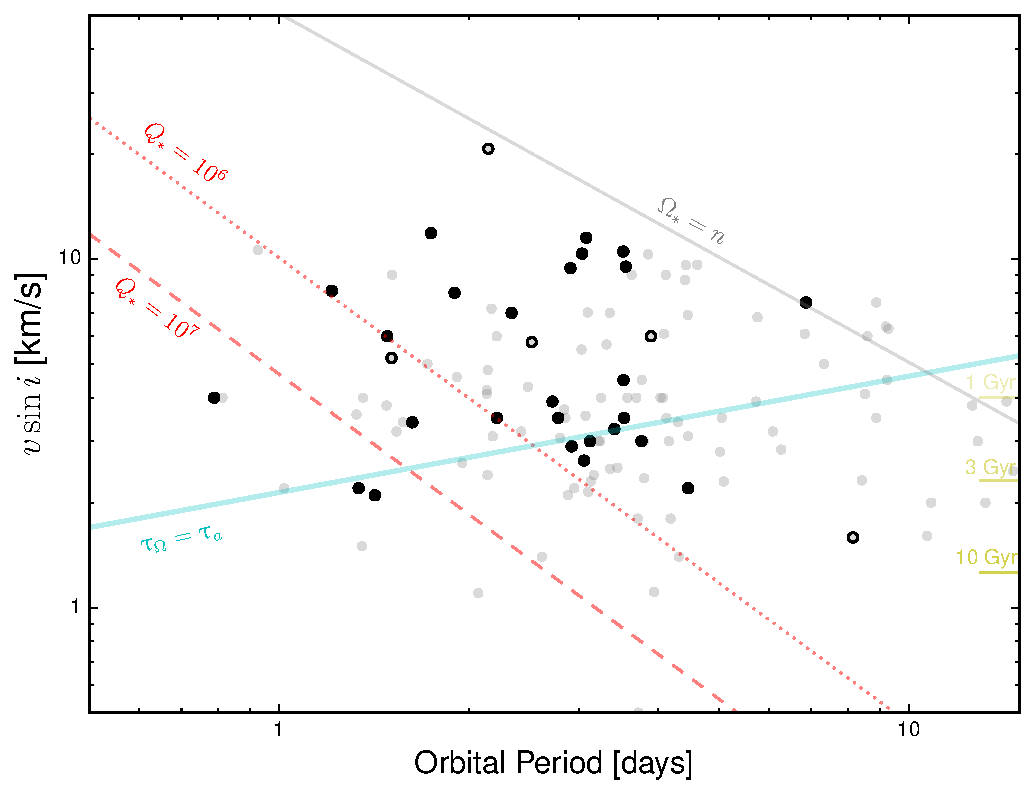
\includegraphics[width=1.0\textwidth]{figures/chapter4/fig10a_cold.pdf}
\caption{类太阳主星与其热类木星的 $v\sin i $---$P$ 图。由于这部分稍冷的恒星受星风与潮汐的同时影响,因此首先我们在右侧纵轴上分别标注了 $V_\tif{s}$ 在不同恒星年龄($\tau_\tif{s} = 1,\,3,\,10$ Gyr,见公式 \ref{eq:wind})的值。灰色的实线代表类太阳恒星的旋同步曲线($\Omega_\tif{s} = n$),在此线的下方则表示行星的潮汐作用会使得行星的轨道收缩而恒星的自转加速。蓝色的实线表示 $L \simeq 2S$,也即轨道演化时标与自转轴演化时标相当($\tau_a = \tau_\Psi$)。红色的虚线表示不同的恒星 $Q$ 值下的潮汐星风平衡态(公式 \ref{eq:lmeq}),点的标记和图 \ref{fig:hotqq} 一致。}
\label{fig:coldevo}
\end{figure}

虽然有了公式 \label{eq:lmeq} 来定定义最终星风、潮汐的合并演化态,但是某些年轻的恒星也许并不能达到
上述状态。该时间在量级上约为 $t_0(V_0/V_e)^2$,因而对于这部分低质量恒星而言,既需要满足能够使得
他们演化至平衡态(特别是 $\Psi$ 角的演化),而且还要保证周围的行星能够被我们观测到。故从公式 
\ref{eq:qspin} 出发,我们重新定义了自转状态的潮汐演化临界值如下:

\begin{equation} \label{eq:lmqspin}
Q_\tif{s}^{\prime} < Q_\tif{spin} \equiv \bigg( 
\frac{9G M_\tif{s}t_0}{4 \gamma_\tif{s}R_\tif{s}^2V_0} \bigg) 
\bigg( \frac{M_\tif{p}}{M_\tif{s}} \bigg)^2  
\bigg( \frac{t}{\tau_\tif{s}} \bigg)^{3/2} \bigg( \frac{R_\tif{s}}{a} \bigg)^6.
\end{equation} %\myequation{低质量恒星自转演化潮汐参数临界值}

从而,在恒星自转减速($Q_\tif{spin} \propto t^{3/2}$)的同时,公式 \ref{eq:lmqspin} 也将变得越来越容
易被满足,因而此自转潮汐参数值为恒星真实值的上限。

\begin{figure}[t]
\centering
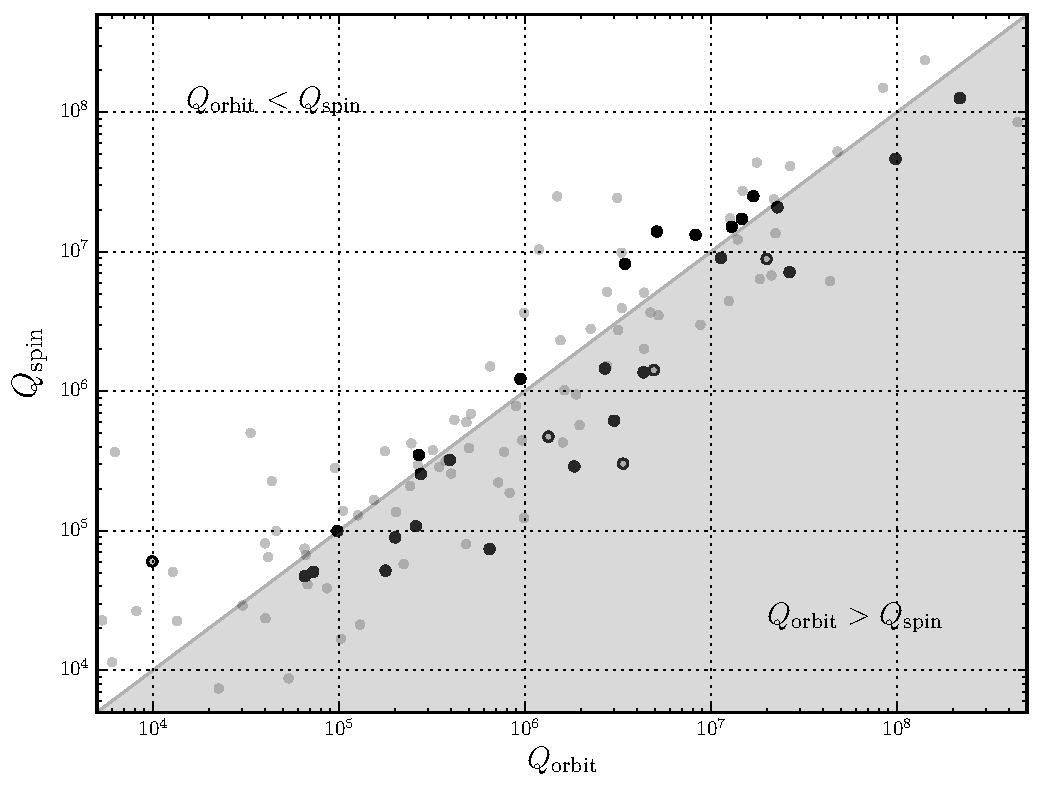
\includegraphics[width=1.0\textwidth]{figures/chapter4/fig10b_cold.pdf}
\caption{与图 \ref{fig:hotqq} 类似的,此为低温恒星的 $Q_\tif{orbit}$ 与 $Q_\tif{spin}$ 分布图。我们对所有系统采用了 $\tau_\tif{s} = 4$ Gyr 的恒星年龄,该值的不确定度则为会导致数据点朝着与对角线( $Q_\tif{spin} = Q_\tif{orbit}$)平行的方向平移。与热恒星周围类似的是,这些系统不太可能在轨道显著变化的同时改变恒星的自转轴方向。} 
\label{fig:coldqq}
\end{figure}


我们将类太阳主星的自转速度 $v\sin i$ 与行星的周期 $P$ 画在图 \ref{fig:coldevo} 中,点的含义与前文中图 \ref{fig:hotqq} 中保持一致。首先可以看出来在这类系统中,主星的自转速度与行星的周期并没有相关性。与
热恒星相比,这部分系统主星的自转速度明显首星风的影响而更小。然而尽管这些恒星的星风效应,绝大部
分系统依然在平衡状态之上($L=2S$),即这些行星在共转半径(灰色线)之内的同时,$L<2S$。由于这
些行星在共转半径之内,因此行星会持续不断的通过潮汐损失角动量来加速恒星自转(以和星风抗衡),从
而轨道不断收缩直到主星内部。

另外该图右侧纵轴上不同年龄的星风损失率也说明了这一点,可以看到在典型的太阳年龄($\tau_\tif{s} \sim 
\tau_\odot \simeq 4 $ Gyr)时刻,星风对恒星角动量损失后的自转速度值已经明显低于现如今观测到的绝大
部分系统,这也说明了潮汐在此类系统中的确起到了一定的作用。然而折中潮汐作用并没有体现在对 $\Psi$
的演化上,因为并不能看到 $\Psi > 30^\circ$ 的实心黑点系统与空心黑点系统之间的系统性差异。所以,我
们将此类系统的 $Q_\tif{orbit}$ 与 $Q_\tif{spin}$  画在了图 \ref{fig:coldqq} 中,可以看到大部分系统主星的
潮汐演化 $Q$ 参数并没有落在允许的区域( $Q_\tif{orbit} < Q_\tif{spin}$ )内,这也说明了潮汐在对这些系
统的演化起作用的期间,却无法从物理上同时允许自转---轨道也一起被影响。

\subsection{总结与讨论}

自转---公转夹角的测量为我们打开了一扇新的检验热木星形成机制的窗口。在对于热木星究竟是通过盘迁移
模型还是高偏心率迁移的模型而形成的争辩上,双方均各执一词。如图 \ref{fig:som2th} 所示,从传统的行星
形成模型出发,行星系统的轨道角动量方向一般被认为与原初行星盘的方向一致,并且恒星自转轴也一同取
向。这在冷恒星周围看到了,但是在热恒星周围却明显不一致($\Psi > 0$)。其中一种理论解释认为无论对
于那种恒星,由于它们周围的热木星的形成过程为高偏心率迁移过程,因此它们周围行星的初始 $\Psi$ 角总
是随机分布在空间内,但由于潮汐作用在低质量恒星(对流外包层)的耗散效率要比在中等质量恒星(辐射
外包层)大得多,因而才会有如此的观测现象\cite{Albrecht2012}。但是从图 \ref{fig:hotqq} 和 \ref{fig:coldqq} 
中我们发现:

\begin{figure}[t!]
\centering
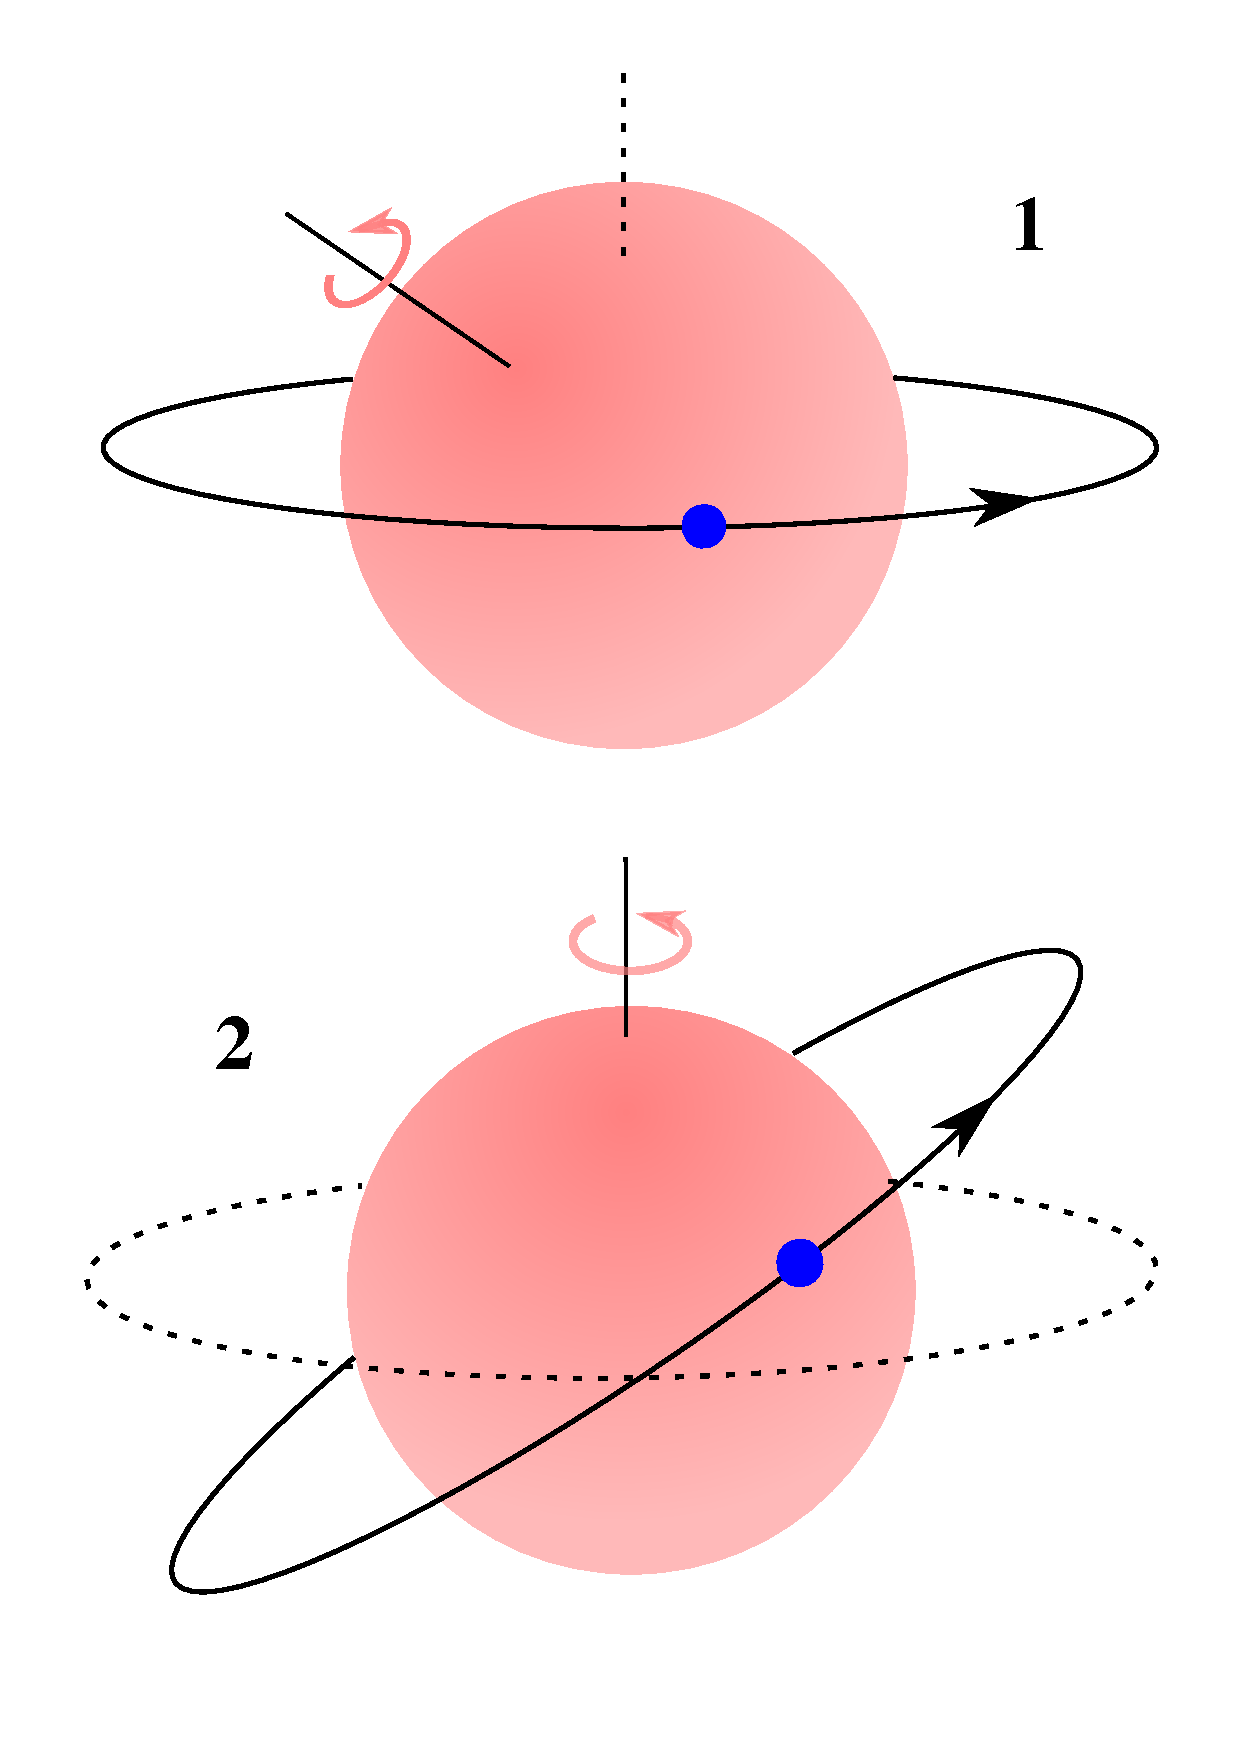
\includegraphics[height=0.85\textheight]{figures/chapter4/fig11_som2th.pdf}
\caption{自转---轨道的指向两种主流解释的示意图。\textbf{1.} 行星轨道取向与主星的自转角动量均保持在原初角动量的位置,有效温度较高的主星的自转轴通过 IGW 激发并改变取向,从而导致观测中的非零 $\Psi$ 角,该理论中的 HJs 往往通过盘迁移而形成,且不依赖于潮汐耗散;\textbf{2.} 行星公转与主星的自转在形成时保持一致,然而由于高偏心率迁移过程中行星的轨道取向被改变,从而导致类太阳恒星系统中有效的潮汐耗散而重新将 $\Psi$ 角减小。}
\label{fig:som2th}
\end{figure}

\begin{enumerate}
\item 没有任何迹象表明 $\Psi$ --- $Q_\tif{spin}$ 具有潮汐效应导致的相关性。因为潮汐作用较强的系统(
$Q < Q_\tif{spin}$ )并没有与 $\Psi$ 接近于零的系统呈现相关。
\item 绝大数系统在图中的「禁区」,即 $Q_\tif{orbit} > Q_\tif{spin}$。在平平衡潮模型下,这些系统 $\Psi$ 
的演化时标要远大于 $a$ 的时标($\tau_a < \tau_\Psi$),这些系统的行星在完成对主星自转轴的重新潮汐
化指向时轨道已经演化至小于主星半径的轨道上。而且对于少部分沿着对角线( $Q_\tif{orbit} = Q_\tif{spin}$)
的系统,它们的 $Q$ 值也是有很大的弥散,因此不能用同样一个潮汐参数来描述所有的系统。
\item 对于大部分观测到了热木星的系统,正说明它们的主星的潮汐参数 $Q$ 的值会在 $10^{4-8}$ 之间分布。
这样的分布与主星的有效温度没有必然关联。并且处于轨旋同步轨道以内($\Omega < n$)的系统,当前观
测到的行星位置极有可能不是它们的最终潮汐演化的结果\cite{Schlaufman2010}。本文得到的 $Q_\tif{orbit}$
只是该系统的最小可能值。对于处于轨旋同步之外的热木星系统,由于它们向外迁移,因此此 $Q_\tif{orbit}$
($10^{6-8}$)则为观测值上限。
\end{enumerate}


在我们的计算中,并没有考虑恒星自转速度中的 $i$ 带来的简并。恒星的年龄也只假定为统一值,类太阳恒
星的星风作用弥散度也未考虑。$\gamma_\tif{s}$ 对热恒星影响并不大,但是在类太阳恒星的内部可能会最
多差至一个量级。虽然如此,在测量恒星自转轴\cite{Hirano2012}以及 $\Psi$ 角度的绝对值上,星震学可能
会大有作为\cite{Chaplin2013,Benomar2014},而测光中黑子与行星的互掩\cite{Desert2011,Nutzman2011,
SanchisOjeda2011}以及恒星自转效应如引力昏暗\cite{Barnes2011,Szabo2011}也会对打破这些值的角度简
并大有用武之地。

值得一提的是,Mazeh 于 2015 年发现类太阳恒星周围的长周期行星也拥有比较一致的自转与轨道法向取向
\cite{Mazeh2015}。而在潮汐作用中,能量耗散与角动量转移的强度十分依赖于行星的半长径 $a$,因此高
偏心率迁移理论以及后续的潮汐作用并不能解释此类系统。另外对于热木星周围的伴星存在肯可能性,一些
巡天显示在这些 HJs 系统周围并没有找到额外的行星级或恒星级伴星\cite{Schlaufman2016,Knutson2014}。
在这样的背景下,也许 Triaud 于 2010 年提出高偏心率迁移来解释这类系统并不必定可取\cite{Triaud2010}。

而对于图 \ref{fig:som2th} 中第二种解释机制\cite{Rogers2012},并不要求潮汐在产生公转---自转不重叠上
起主导作用,因此也是非常有前景的解释。比如 Triana 近期提出通过星震学探测由于 IGW 产生的较差自转
现象,纬度方向上的较差自转和自转轴指向的变化也同样可能在这些热木星系统的主星上被探测到
\cite{Triana2015}。



